\appendix
\FloatBarrier
\section{Hardware and Software}\label{appendix:Hardware}
All numerical simulations were done on one of two machines,
\begin{itemize}
    \item [(M1)] Lenovo NeXtScale server BEAR HPC (Birmingham Environment for Academic Research High Performance Computing) processing unit (CPU), using 2x Intel(R) Xeon(R) Platinum 8360Y CPU  (each with 36 cores @ 2.40GHz) and 64 GB DDR4 RAM.
    \item [(M2)] Lenovo Thinkstation, with 2x Intel Xeon 4116 CPUs (each with 12 cores @ 2.10GHz), 128 GB DDR4 RAM, and an NVIDIA Quadro RTX 5000 GPU (3072 parallel-processing cores, 16 GB GDDR6 RAM).
\end{itemize}
(M1) forms part of a HPC cluster but all computation will be limited to a single compute node per simulation. Most simulations here were limited to 20 computation threads on (M1) and 4 on (M2) unless otherwise stated.

For data accessibility all Matlab code to generate all data and figures found in this paper can be found at \url{https://github.com/Walkersb101/KIFMM}.

\FloatBarrier
\section{Generalised Minimum RESidual method}\label{appendix:GMRES}
\sectionmark{GMRES}

The Generalised Minimum RESidual method (GMRES) \cite{Saad1986GMRES:Systems} is a iterative method based on Krylov methods for solving the System $A\bm{x}=\bm{b}$ where $A$ is an arbitary non-symmetric matrix of order $n$ and $\bm{b}$ is a known vector of order $n$. Krylov methods generate a Krylov subspace through repetitively performing vector matrix multiplication involving $A$. This allows for the computation of large systems where operations of order $\mathcal{O}(N^3)$ are too large to compute the matrix inverse, or where we are unable to form the matrix but can compute the matrix vector product as in the Kernel Independent Fast Multiple Method (KIFMM) (\cref{sec:KIFMM}) \cite{Ipsen1998TheMethods}.

The GMRES method finds find the solution $\bm{y}_k$ at each iteration $k \geq 1$ from the subspace
\begin{equation*}
    \mathcal{K}_k(A,v^{(0)}) = \text{span}(\bm{v}^{(0)},A\bm{v}^{(0)},A^2\bm{v}^{(0)},\dots,A^{k-1}\bm{v}^{(0)})
\end{equation*}
where $\bm{v}^{0}$ is the normalised vector of the residual $\bm{r}^{(0)}=\bm{b}-A\bm{x}^{(0)}$ which reduces the residual to the least square problem $\min\limits_{x\in\mathcal{K}(A,b)} \lVert b-Ax \rVert$.

When no initial guess for $\bm{x}^{(0)}$ is given we have that $\bm{r}^{(0)}=b$, experimental results for methods where an initial guess is provided can be seen in \cref{sec:Guess}. GMRES solves this least square problem through the use of a orthogonal basis $\{\bm{v}^{(1)},\bm{v}^{(2)},\dots,\bm{v}^{(k)}\}$ for $\mathcal{K}(A,b)$, this is constructed using Arnoldi's method \cite{Arnoldi1951TheProblem,Elman2005FiniteDynamics}. The $k+1$ subspace is constructed from the $k$ subspace by orthogonalising the vector $A\bm{v}_K$ against $\mathcal{K}_k(A,v^{(0)})$ subspace. This is done by
\begin{equation*}
    \bm{\hat{v}}_{k+1} = A\bm{v}_k - (h_{1,j}\bm{v}_1 + \dots + h_{j,j}\bm{v}_j)
\end{equation*}
where $h_{ij} = v_j^*Av_j$ and $v_j^*$ is the conjugate transpose of $v_j$. We then normalise $\bm{\hat{v}}_{k+1}$ to obtain $\bm{v}_{k+1}=\bm{\hat{v}}_{k+1}/\lVert \bm{\hat{v}}_{k+1} \rVert$
By collecting the basis vectors in a matrix $V_k = [\bm{v}^{(1)},\bm{v}^{(2)},\dots,\bm{v}^{(k)}]$ we get that the decomposition from Arnoldi's method as
\begin{equation*}
    AV_j = V_{j+1} H_j
\end{equation*}
 where $H_j$ is an upper Hessenberg matrix of size $j + 1\times j$ formed by $\hat{H}_k = [h_{ij}]_{1 \leq i \leq k+1, 1 \leq j \leq k}$. As our solution to the least square problem is in $\mathcal{K}_k(A,r^{(0)})$ then we can write it as $V_k\bm{y}^{(k)}$ for some vector $\bm{y}^{(k)}$. This means we can rewrite the least square problem in terms of $H_k$ as
 \begin{equation*}
 \begin{aligned}
          \beta_k &= \min\limits_{\bm{y}^{(k)}} \lVert  \beta_0 \bm{v}_0 - AV_k\bm{y}^{(k)} \rVert \\
          &= \min\limits_{\bm{y}^{(k)}} \lVert \beta_0 V_{k+1} \bm{e}_1 - V_{k+1}H_k\bm{y}^{(k)} \rVert \\
          &= \min\limits_{\bm{y}^{(k)}} \lVert \beta_0 \bm{e}_1 - H_k\bm{y}^{(k)} \rVert
 \end{aligned}
 \end{equation*}
where $\bm{e}_1 = [1,0,\dots,0]^T$. This process is repeated until $\beta_k$ is under some relative tolerance $\tau$ specified. The final estimation for $\bm{x}$ is therefore constructed from $\bm{x}^{(k)} = \bm{x}^{(k)} + V_k\bm{y}^{(k)}$.
\begin{algorithm}
\caption{The GMRES Algorithm}\label{alg:GMRES}
\begin{algorithmic}[1]
\State Choose $\bm{x}^{(0)}$, compute $\bm{r}^{(0)}=\bm{b}-A\bm{x}^{(0)}$, $\beta_0 = \lVert \bm{r}^{(0)} \rVert$, $\bm{v}^{(0)} = \bm{r}^{(0)}/\beta_0$
\For{$k = 1,2,\dots \textbf{ Until } \beta_k < \tau \beta_0$}
\State $\bm{w}_0^{(k+1)} = Av^{(k)}$
\For{$l = 1$ to $k$}
\State $h_{lk}=\langle \bm{w}_l^{(k+1)}, \bm{v}^{(l)} \rangle$
\State $\bm{w}_{l+1}^{(k+1)} = \bm{w}_l^{(k+1)} - h_{lk}\bm{v}^{(l)}$
\EndFor
\State $h_{k+1,k}=\lVert \bm{w}_{k+1}^{(k+1)} \rVert$
\State $\bm{v}^{(k+1)} = \bm{w}_{k+1}^{(k+1)}/h_{k+1,k}$
\State Compute $\bm{y}^{(k)}$ such that $\beta_k = \lVert \beta_0 \bm{e}_1 - H_k  \bm{y}^{(k)} \rVert$ is minimised, where
\State $H_k = [h_{ij}]_{1 \leq i \leq k+1, 1 \leq j \leq k}$
\EndFor
\State $\bm{x}^{(k)} = \bm{x}^{(k)} + V_k\bm{y}^{(k)}$, where $V_k = [\bm{v}^{(1)},\bm{v}^{(2)},\dots,\bm{v}^{(k)}]$
\end{algorithmic}
\end{algorithm}

GMRES will converge on the least square solution in at most $n$ iterations, although it will often converge to small values of $\beta_k$ in f steps. The exact number of iterations is correlated closely with the  condition of the matrix $A$ where better conditioned matrices will converge faster. In slow converging systems, where the number of iterations $k$ that are required to converge to the required tolerance $\tau$ is large and can result in large computation and storage requirements as the new vector $\bm{v}_{k+1}$ needs to be orthogonalised against all previous vectors in the basis. This means that the computation and storage requirements for the GMRES algorithm grow at a rate of $\mathcal{O}(kn)$. An adaption to the algorithm denoted GMRES($m$) is used where after $m$ iterations the best guess $\bm{u}^{(m)}$ is constructed and used in place of $\bm{u}^{(0)}$ as the initial guess. This provides a upper bound on the computation and storage requirement of the algorithm although may slow down convergence as each approximation is built using a smaller Krylov subspace.

\FloatBarrier
\section{Tree Traversal}\label{appendix:Tree}
In this section we will give a brief overview of the two tree traversals needed to perform the fast multiple algorithm. We will consider a simple binary tree where each node had two children nodes. If we consider the binary tree in \cref{fig:BlankTree}, then we can consider both pre and post order traversals.
\begin{figure}[ht]
    \centering
    \resizebox{.4\linewidth}{!}{\begin{tikzpicture}
    \node[anchor = south west,inner sep=0] (image) at (0,0) {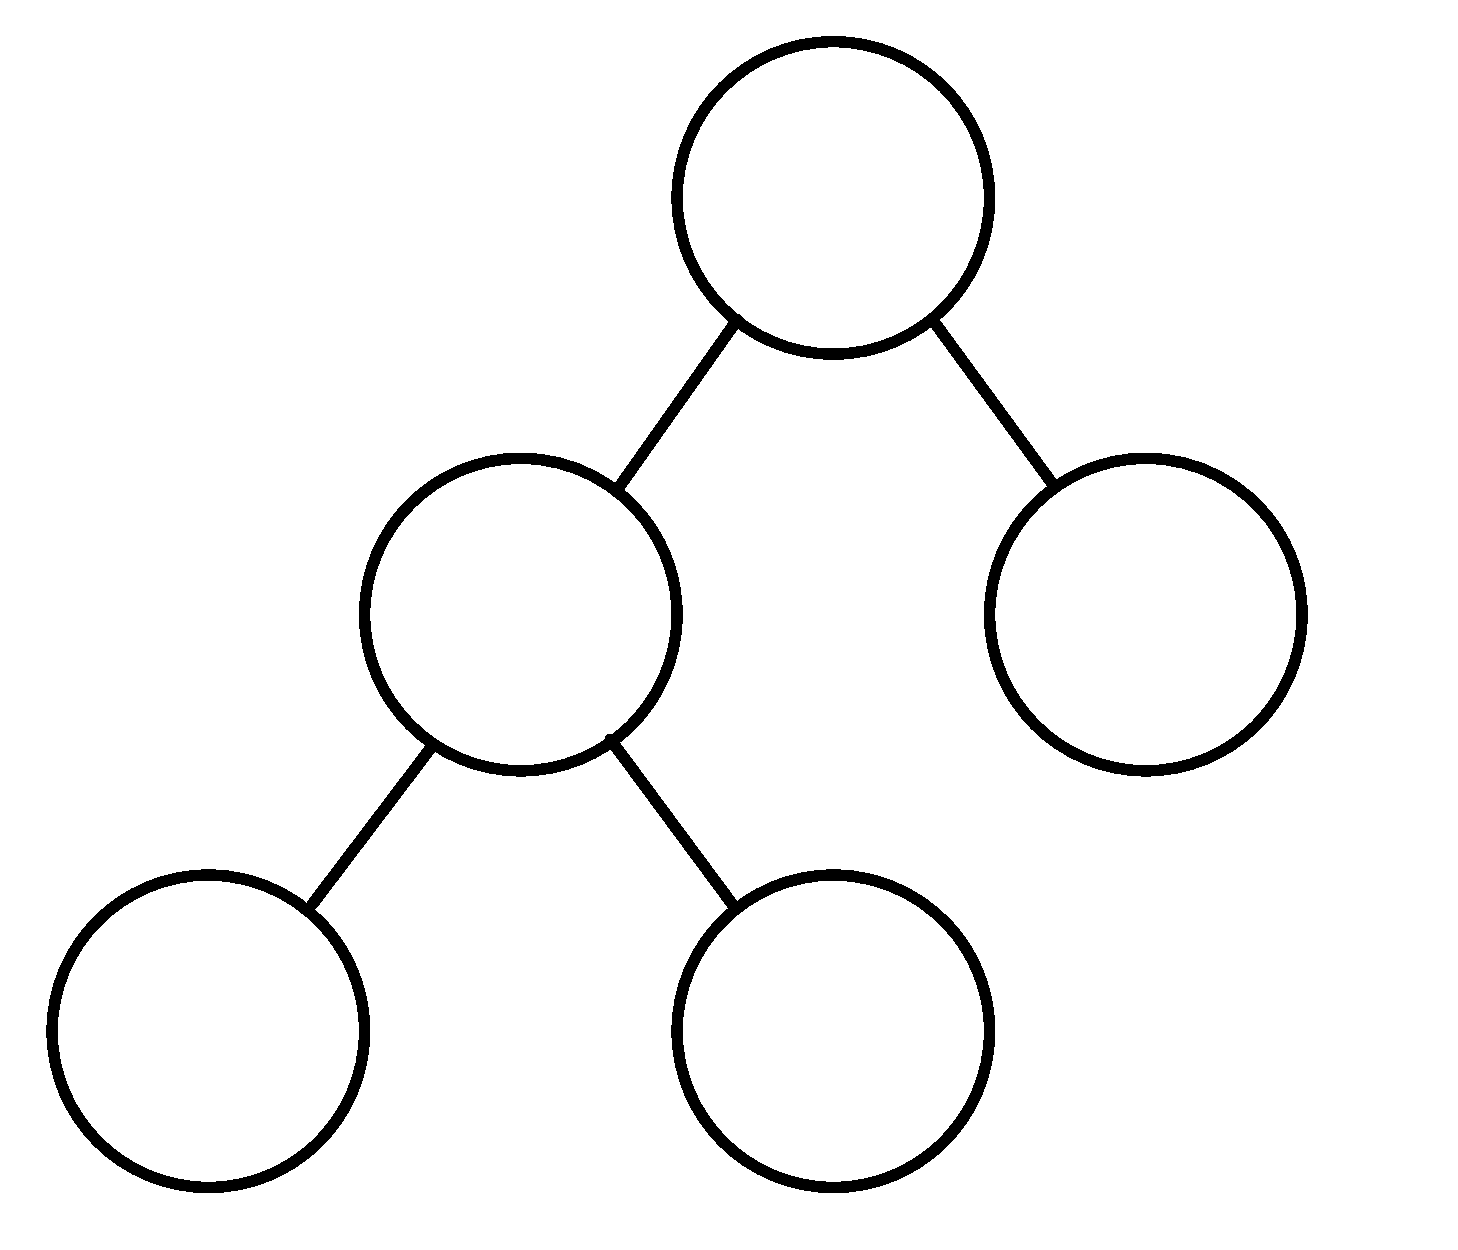
\includegraphics[width=.6\textwidth]{Images/TreeTraversal/BlankTree.pdf}};
    \begin{scope}[x={(image.south east)},y={(image.north west)}]
    \begin{scope}[x={(image.south east)},y={(image.north west)}]
        \node at (0.57,0.83) {\Huge $1$};
        \node at (0.36,0.51) {\Huge $2$};
        \node at (0.78,0.51) {\Huge $3$};
        \node at (0.14,0.17) {\Huge $4$};
        \node at (0.57,0.17) {\Huge $5$};
    \end{scope}
    \end{scope}
\end{tikzpicture}}
    \caption{A simple tree structure}
    \label{fig:BlankTree}
\end{figure}
The post order traversal is used in cases where we need to look at all the children of a node before looking at the node itself. This is useful for example in the upwards pass of the fast multipole method, where we need to compute the upwards equivalent surface of all nodes before computing the upwards equivalent surface of the node itself with the multipole to multipole translation (eq.~\ref{eq:M2M}). For the case of the binary tree in \cref{fig:BlankTree}, we traverse the nodes in the order $4, 5, 2, 3, 1$ with the path taken displayed in \cref{fig:Postorder}.

Another way in which we can traverse tree structures in the pre order traversal where we work our way down from the root of the tree. We use this in fast multipole methods so we can use local to local translation (eq.~\ref{eq:L2L}). The pre order traversal differs from post order traversal as, in this case, we visit the current node first before recursively traversing each subtree. For example the tree in \cref{fig:BlankTree} can be traversed using pre order traversal in the order $1, 2, 4, 5, 3$ as illustrated in \cref{fig:Preorder}.

For application of both traversals to an octtree, where we traverse each subtree individually, the order in which each subtree is traversed does not matter and only comes down to convention, however we do need to make sure that every subtree is traversed for each node.

\begin{algorithm}
\caption{Binary Post Order Traversal}
\begin{algorithmic}[1]
\State Recursively traverse the current node's left subtree
\State Recursively traverse the current node's right subtree
\State Visit the current node.
\end{algorithmic}
\end{algorithm}

\begin{algorithm}
\caption{Binary Pre Order Traversal}
\begin{algorithmic}[1]
\State Visit the current node
\State Recursively traverse the current node's left subtree
\State Recursively traverse the current node's right subtree.
\end{algorithmic}
\end{algorithm}

\begin{figure}
     \centering
     \begin{subfigure}[b]{0.4\textwidth}
         \centering
         \resizebox{\linewidth}{!}{\begin{tikzpicture}
    \node[anchor = south west,inner sep=0] (image) at (0,0) {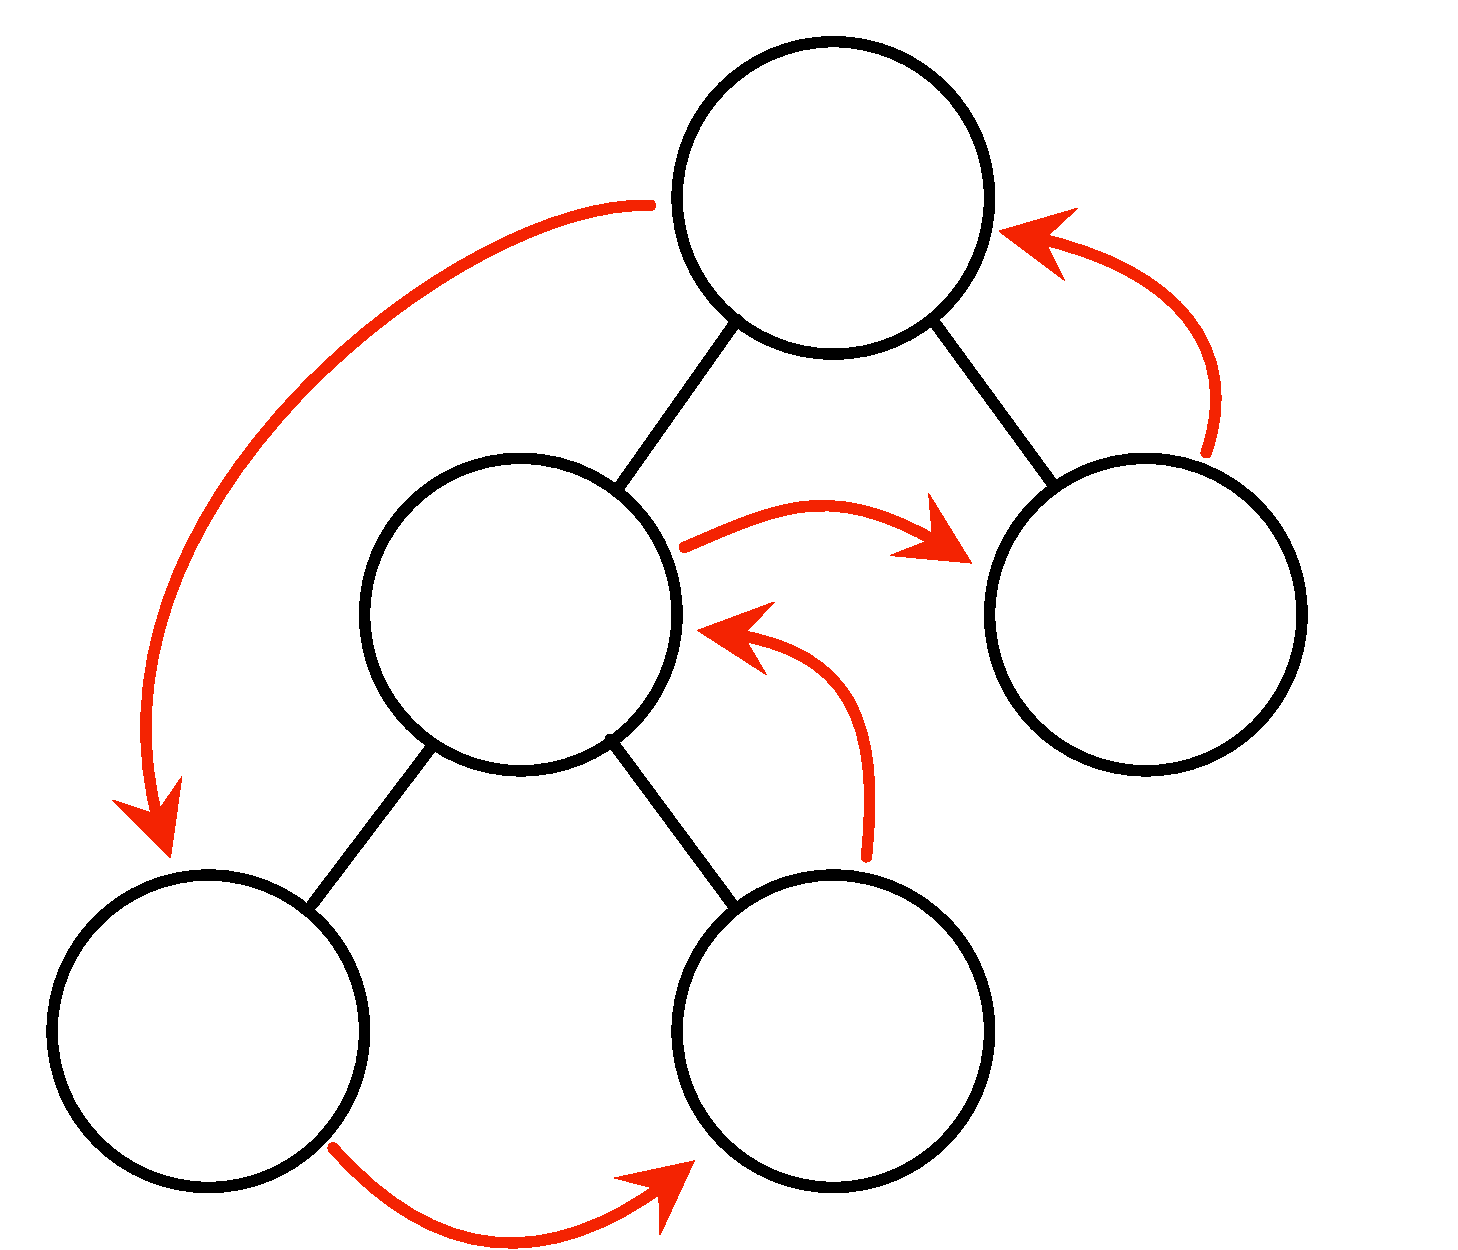
\includegraphics[width=.6\textwidth]{Images/TreeTraversal/Postorder.pdf}};
    \begin{scope}[x={(image.south east)},y={(image.north west)}]
    \begin{scope}[x={(image.south east)},y={(image.north west)}]
        \node at (0.57,0.83) {\large $1$};
        \node at (0.36,0.51) {\large $2$};
        \node at (0.78,0.51) {\large $3$};
        \node at (0.14,0.17) {\large $4$};
        \node at (0.57,0.17) {\large $5$};
    \end{scope}
    \end{scope}
\end{tikzpicture}}
         \caption{Diagram showing post order tree traversal}
         \label{fig:Postorder}
     \end{subfigure}
          \hfill
     \begin{subfigure}[b]{0.4\textwidth}
         \centering
         \resizebox{\linewidth}{!}{\begin{tikzpicture}
    \node[anchor = south west,inner sep=0] (image) at (0,0) {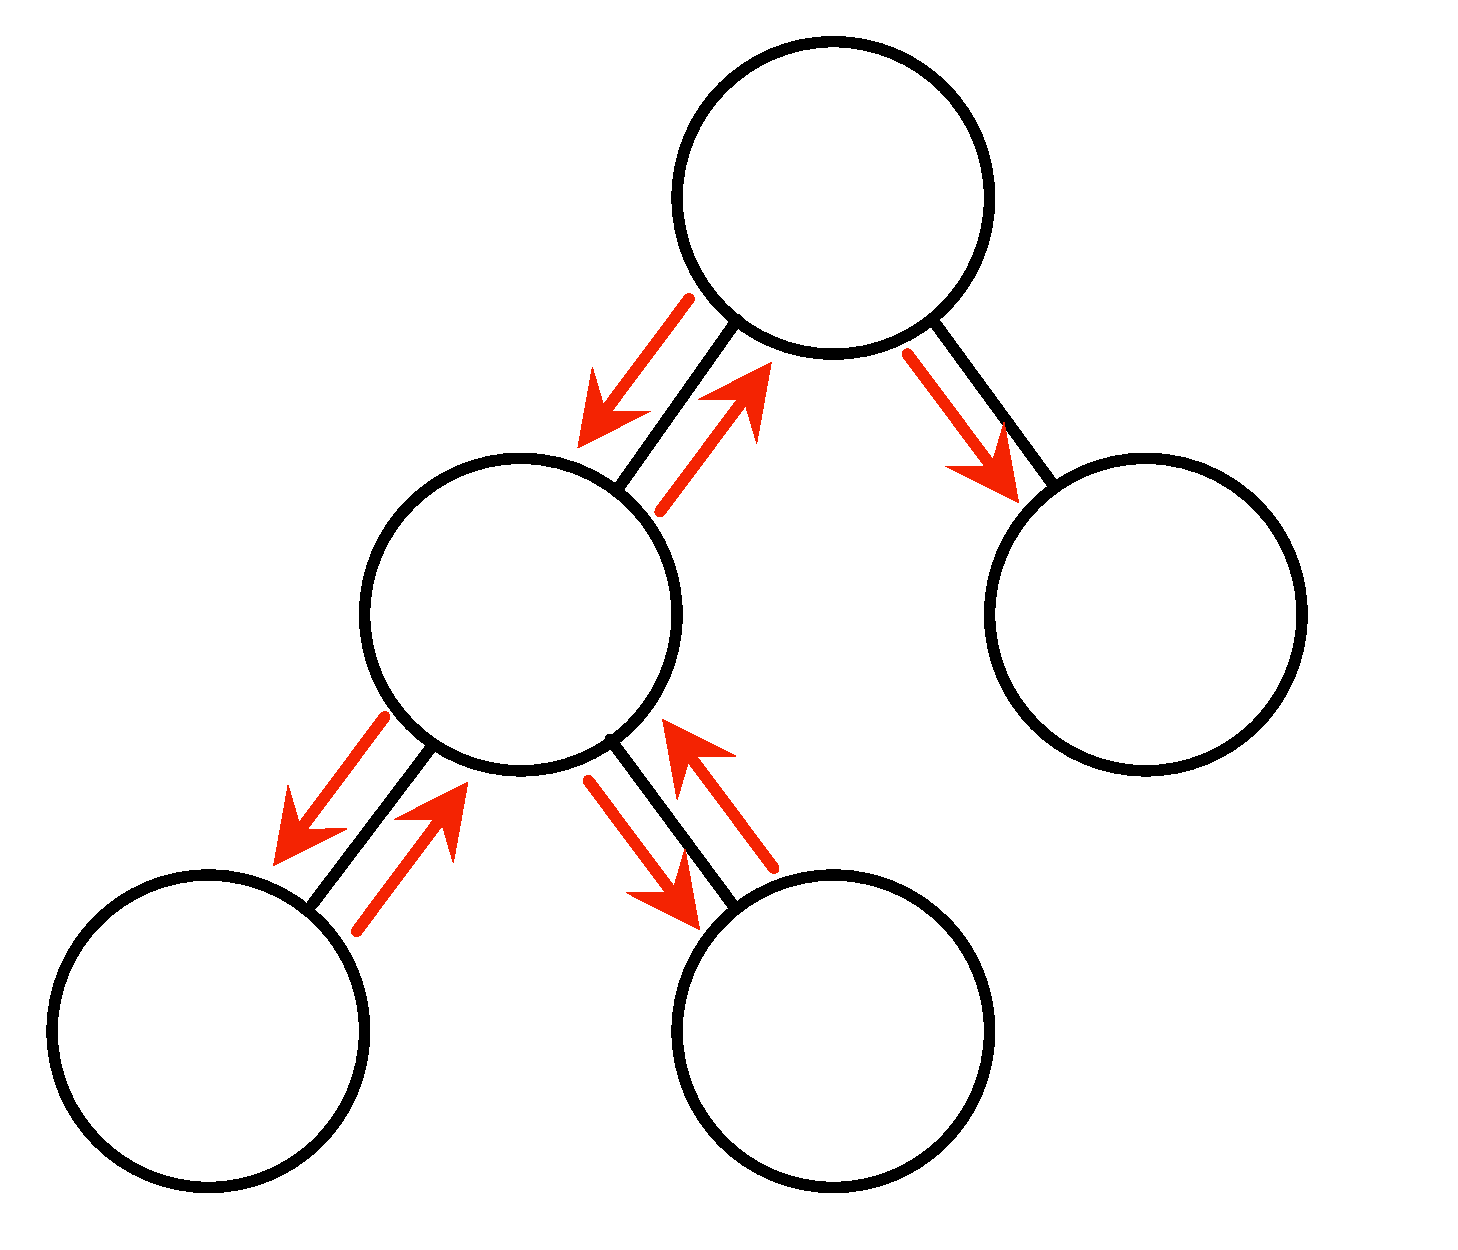
\includegraphics[width=.6\textwidth]{Images/TreeTraversal/Preorder.pdf}};
    \begin{scope}[x={(image.south east)},y={(image.north west)}]
    \begin{scope}[x={(image.south east)},y={(image.north west)}]
        \node at (0.57,0.83) {\large $1$};
        \node at (0.36,0.51) {\large $2$};
        \node at (0.78,0.51) {\large $3$};
        \node at (0.14,0.17) {\large $4$};
        \node at (0.57,0.17) {\large $5$};
    \end{scope}
    \end{scope}
\end{tikzpicture}}
         \caption{Diagram showing pre order tree traversal}
         \label{fig:Preorder}
     \end{subfigure}
        \caption{Diagrams showing Pre and Post order traversal of the tree defined in \cref{fig:BlankTree}}
        \label{fig:TreeTraversal}
\end{figure}


\FloatBarrier
\section{Nyström Swimming Problem} \label{appedix:NystromSwim}
The Nyström discretisation of \cref{eq:swimmingProblem,eq:swimmingProblemBnd,eq:swimmingProblemMulti} can be seen below. 

\subsection{Single swimmer}
For a single swimmer with no boundaries (eq.~\ref{eq:swimmingProblem}) the problem takes the form as 
\begin{equation*}
\begin{gathered}
    -U_{i}-\epsilon_{i j k} \Omega_{j}\left(x_k[{m}]-x_{0 k}\right)+\frac{1}{8 \pi\mu} \sum_{n=1}^N S_{i j}^{\epsilon}(\bm{x}_m, \bm{x}_n) f_{j}(\bm{x}_n) A_n =  B_{i j} \dot{\xi}_{j}[m] \\ \text { for all } m = 1,\dots,N\\
    \sum_{n=1}^N f_{i}(\bm{x}_n) A_n=0 \\
    \sum_{n=1}^N \epsilon_{i k j} (x_{k}[n]-x_{0 k}) f_{j}(\bm{x}_n) A_n=0,
\end{gathered}
\end{equation*}
where $x_{i}[n]$ denotes the the position of the $n$th quadrature point in the $i$th axis and $A_n$ the quadrature weight at the point $\bm{x}_n$. Taking the same block matrix form described in \cref{eq:swimmingStructure} the blocks can be written as
\begin{align*}
A_{ij}(m,n) &= \frac{1}{8\pi\mu} S_{ij}^\epsilon (\bm{x}_m,\bm{x}_{n}) \text { for } m,n = 1,\dots,N \\
B_{i}^{U}(m,j) &= -\delta_{ij} \text { for } m = 1,\dots,N \\
B_{i}^{\Omega}(m,j) &= -\epsilon_{ijk}(x_k[m]-x_{0k}) \text { for } m = 1,\dots,N \\
B_{j}^{F}(i,n) &= \delta_{ij} \text { for } n = 1,\dots,N \\
B_{j}^{M}(i,n) &= \epsilon_{ikj} (x_k[n]x_{0 k}) \text { for } n = 1,\dots,N
\end{align*}

\subsection{Boundaries}
Recalling the same notation described in \cref{sec:boundries} the block matrix components of \cref{eq:swimmingStructure} can be written in the case of the Nyström discretisation as,
\begin{align*}
A_{ij}(m,n) &= \frac{1}{8\pi\mu} S_{ij}^\epsilon (\bm{x}_m,\bm{x}_{n}) \text { for } m,n = 1,\dots,N_s,N_D+1,\dots,N_D+N_B \\
B_{i}^{U}(m,j) &= \begin{cases} -\delta_{ij} \text { for } m = 1,\dots,N_D \\ 0 \text { for } m = N_D+1,\dots,N_D+N_B\end{cases} \\
B_{i}^{\Omega}(m,j) &= \begin{cases} -\epsilon_{ijk}(x_k[m]-x_{0k}) \text { for } m = 1,\dots,N \\ 0 \text { for } m = N_D+1,\dots,N_D+N_B\end{cases} \\
B_{j}^{F}(i,n) &= \begin{cases} \delta_{ij} \text { for } n = 1,\dots,N \\ 0 \text { for } n = N_D+1,\dots,N_D+N_B\end{cases} \\
B_{j}^{M}(i,n) &= \begin{cases} \epsilon_{ikj} (x_k[n]-x_{0 k}) \text { for } n = 1,\dots,N \\ 0 \text { for } n = N_D+1,\dots,N_D+N_B\end{cases}
\end{align*}

\subsection{Multiple Swimmers}
As in the NEAREST case we will consider $N_{sw}$ swimmers which each have collocation points $x_i^{(1)}[\cdot],\dots,x_i^{(N_{sw})}[\cdot]$ where $x_i^{(1)}[\cdot]$ denotes all the $i$th components of the first swimmers collocation points and $x_i^{(B)}[\cdot]$ is the $i$th components of the boundaries collocation points. It is assumed that the same ordering convention is used as in the NEAREST method for all vectors.
Defining the index $\iota(s)=\sum_{\alpha=1}^{s-1}N_D(\alpha)$ for $1<s\leq N_{sw}$ to be the location of the $s$th swimmer in $\bm{x}_i$, and $\iota(1)=1$. The stokeslet matrix is constructed as normal by
\begin{equation*}
    A_{ij}(\alpha,\beta) = \frac{1}{8\pi\mu} S_{ij}^\epsilon (\bm{x}_\alpha,\bm{x}_{\beta}) \text { for } \alpha,\beta = 1,\dots,N_F
\end{equation*}
Defining $\bm{1}^{(n)}$ to be a column vector of ones with length $n$, $\bm{1}^{(n)T}$ to be the transpose of $\bm{1}^{(n)}$ a row vector of ones with length $n$ and $\bm{0}^{(m\times n)}$ to be a $(m\times n)$ matrix of zeros. By defining
\begin{equation*}
\arraycolsep=0.4pt\def\arraystretch{0.75}
    \tilde{x}_i(\cdot,\cdot)=\left(\begin{array}{c}
         \begin{array}{ccc}
             x_i^{(1)}[\cdot]-x_{0i}^{(1)} & & \\
              & \ddots & \\
              & & x_i^{(N_{sw})}[\cdot]-x_{0i}^{(N_{sw})}
         \end{array}\\
         \bm{0}^{(N_B \times N_{sw})}
    \end{array}\right).
\end{equation*}
The translational and rotational components of the matrix can be defined to be
\begin{equation*}
\arraycolsep=0.4pt\def\arraystretch{0.75}
    B^U = \mathds{1}_{3} \otimes \left(\begin{array}{c}
         \begin{array}{ccc}
             -\bm{1}^{(N_D(1))} & & \\
              & \ddots & \\
              & & -\bm{1}^{(N_D(N_{sw}))}
         \end{array}\\
         \bm{0}^{(N_B \times N_{sw})}
    \end{array}\right), \;
    B^\Omega =
    \left(\begin{array}{ccc}
             & -\tilde{x}_3(\cdot,\cdot) & \tilde{x}_2(\cdot,\cdot)\\
            \tilde{x}_3(\cdot,\cdot) & & -\tilde{x}_1(\cdot,\cdot)\\
            -\tilde{x}_2(\cdot,\cdot) & \tilde{x}_1(\cdot,\cdot) &
          \end{array}\right)
\end{equation*}
with $\mathds{1}_{3}$ denoting the $3\times3$ identity matrix and $\otimes$ the Kronecker product. This means that $B^U_i$ and $B_i^\Omega$ remain the same for both discretisation for $i=1,2,3$. 

To construct the $N_{sw} \times N_F$ matrices we define the row vector of size $1 \times N_D(s)$ 
\begin{equation*}
    \chi_j^{(s)}[\cdot] = (x_j(\gamma) - x_{0 j}) \text{ for } \gamma = \iota(s),\cdots,\iota(s+1)-1
\end{equation*}
these allow us to define
\begin{equation*}
\arraycolsep=0.4pt\def\arraystretch{0.75}
    \tilde{\chi}_j(\cdot,\cdot)=\left(\begin{array}{cc}
         \begin{array}{ccc}
             \chi_j^{(1)}[\cdot] & & \\
              & \ddots & \\
              & & \chi_j^{(N_{sw})}[\cdot]
         \end{array} & \bm{0}^{(N_{sw} \times N_B)}
    \end{array}\right).
\end{equation*}
Then
\begin{equation*}
\arraycolsep=0.4pt\def\arraystretch{0.75}
    B^F = \mathds{1}_{3} \otimes \left(\begin{array}{cc}
         \begin{array}{ccc}
             \bm{1}^{(1)T}[\cdot] & & \\
              & \ddots & \\
              & & \bm{1}^{(N_{sw})T}[\cdot]
         \end{array} & \bm{0}^{(N_{sw} \times N_B)}
    \end{array}\right), \;
    B^M =
    \left(\begin{array}{ccc}
             & -\tilde{\chi}_3(\cdot,\cdot) & \tilde{\chi}_2(\cdot,\cdot)\\
            \tilde{\chi}_3(\cdot,\cdot) & & -\tilde{\chi}_1(\cdot,\cdot)\\
            -\tilde{\chi}_2(\cdot,\cdot) & \tilde{\chi}_1(\cdot,\cdot) &
          \end{array}\right)
\end{equation*}
Finally, defining the right-hand side vector as $(\bm{V}_1,\bm{V}_1,\bm{V}_1,\bm{0}_{(6N_{sw} \times 1)})^T$ where
\begin{equation*}
    V_i^{(s)} = (B_{ij}^{(1)}\dot{\xi}_j^{(1)}[\cdot],\dots,B_{ij}^{(N_{sw})}\dot{\xi}_j^{(N_{sw})}[\cdot],\dot{x}_i[1],\dots,\dot{x}_i[N_B])
\end{equation*}
This forms a linear system of $3(N_F+2N_{sw})$ equations in $3(N_F+2N_{sw})$ unknowns in the same structure as \cref{eq:swimmingStructure} as we had for the NEAREST discretisation.

\FloatBarrier
\section{Condition Number}\label{appendix:ConNum}
We investigate the condition number and eignevalue distribution of various matrices derived in the paper. We consider the change in the parameters, two which affect the total number of quadrature points and also the change in $\epsilon$. Spherical swimmers of radius $0.5$ with varying number of quadrature points are randomly scattered, but not allowed to intersect, in a domain of $5 \times 5 \times 5$. 

As expected the larger $\epsilon$ systems are significantly worse conditioned even when preconditioned, we also note an increase in the condition of all matrices as the number of scalar degrees of freedom and swimmers increases, this is due to the spacing between particles becoming smaller and the variation in the magnitude of the interactions becoming larger. 

We also consider the eigenvalues of the 40 swimmers and 114 force quadrature points case to illustrate the effect of eigenvalues on the convergence of the GMRES algorithm. The eigenvalues found use the perfect LU decomposition so the eigenvalues of problem considered in the paper only approximate these solutions and as such do not converge after one iteration as would be expected. 


\begin{figure}[hb]
\caption[Condition of matrices considered in this paper.]{Condition of matrices considered in this paper with various changes in parameter.}
    \begin{subfigure}{0.3\textwidth}
        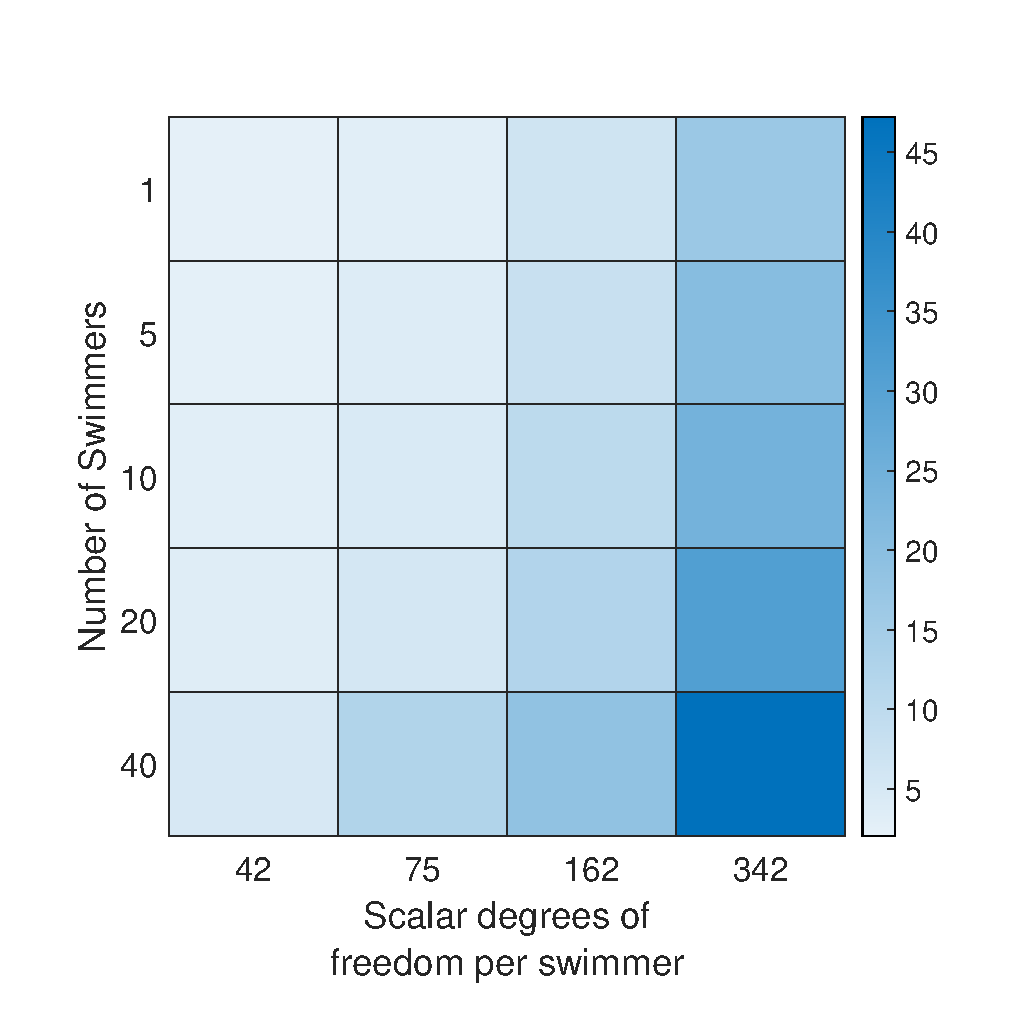
\includegraphics[width=\linewidth]{Images/Condition/Stokeslet Matrix-1.pdf}
        \caption{Nyström Stokeslet Matrix with $\epsilon=1e-1$}
    \end{subfigure}
    \begin{subfigure}{0.3\textwidth}
        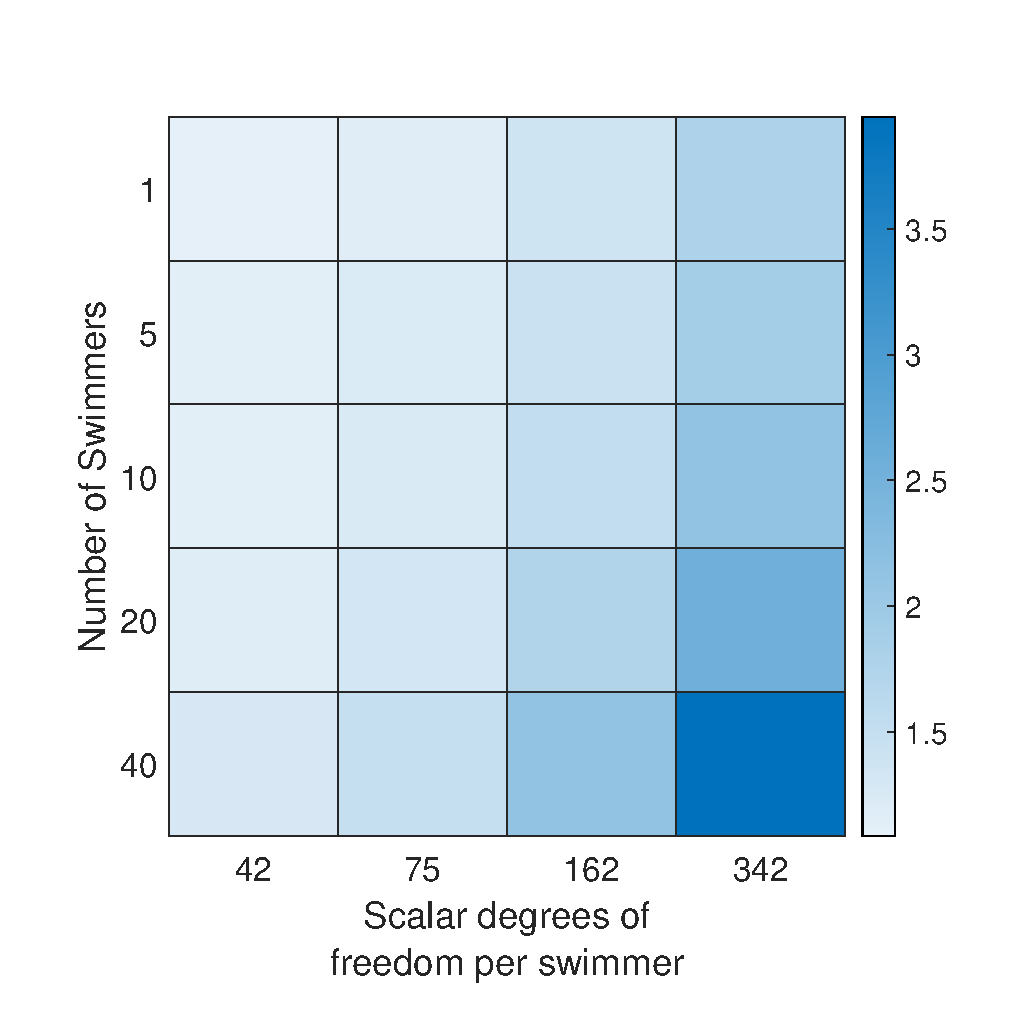
\includegraphics[width=\linewidth]{Images/Condition/Stokeslet Matrix-2.pdf}
        \caption{Nyström Stokeslet Matrix with $\epsilon=1e-2$}
    \end{subfigure}
    \begin{subfigure}{0.3\textwidth}
        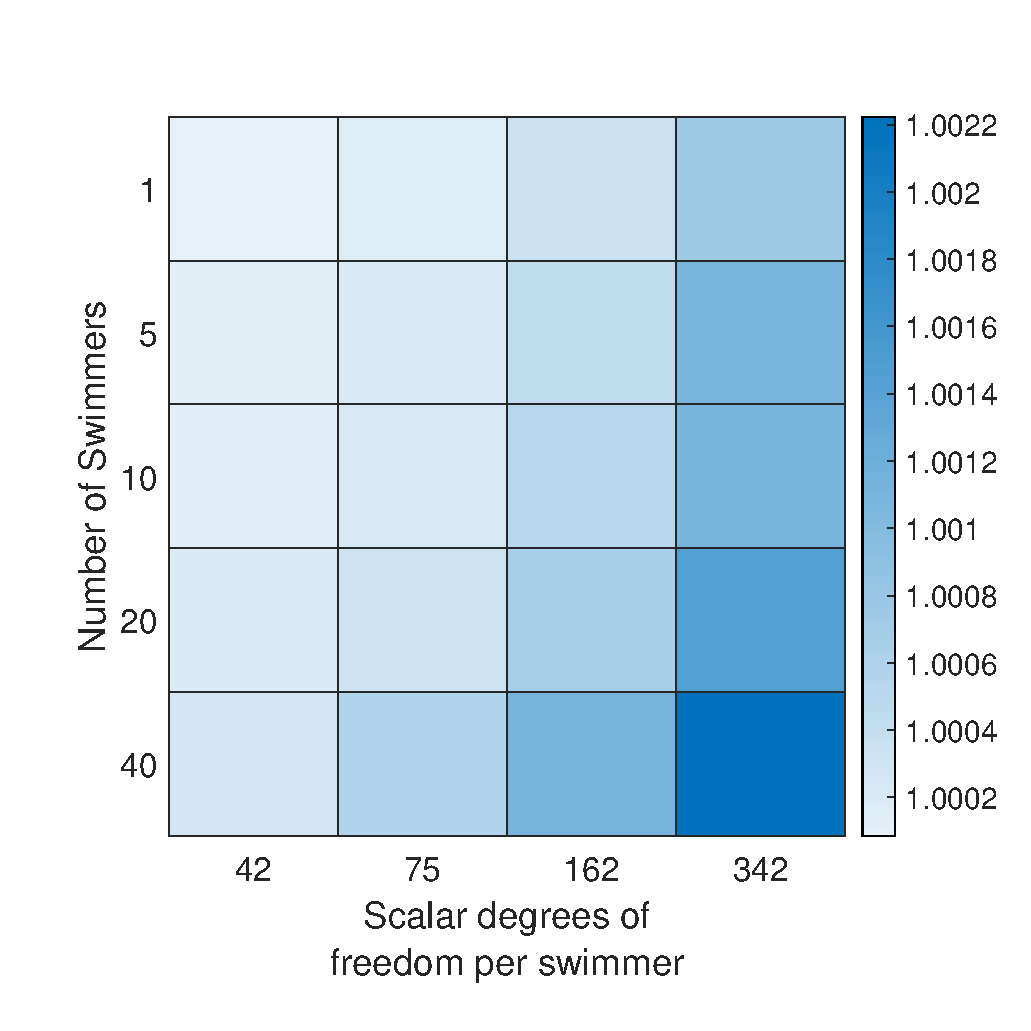
\includegraphics[width=\linewidth]{Images/Condition/Stokeslet Matrix-5.pdf}
        \caption{Nyström Stokeslet Matrix with $\epsilon=1e-5$}
    \end{subfigure}
\end{figure}
\begin{figure}
\ContinuedFloat
    \begin{subfigure}{0.3\textwidth}
        \includegraphics[width=\linewidth]{Images/Condition/Mobility matrix-1.pdf}
        \caption{Nyström Swimming Matrix with $\epsilon=1e-1$}
    \end{subfigure}
    \begin{subfigure}{0.3\textwidth}
        \includegraphics[width=\linewidth]{Images/Condition/Mobility matrix-2.pdf}
        \caption{Nyström Swimming Matrix with $\epsilon=1e-2$}
    \end{subfigure}
    \begin{subfigure}{0.3\textwidth}
        \includegraphics[width=\linewidth]{Images/Condition/Mobility matrix-5.pdf}
        \caption{Nyström Swimming Matrix with $\epsilon=1e-5$}
    \end{subfigure}
\end{figure}


\begin{figure}
\ContinuedFloat
    \begin{subfigure}{0.3\textwidth}
        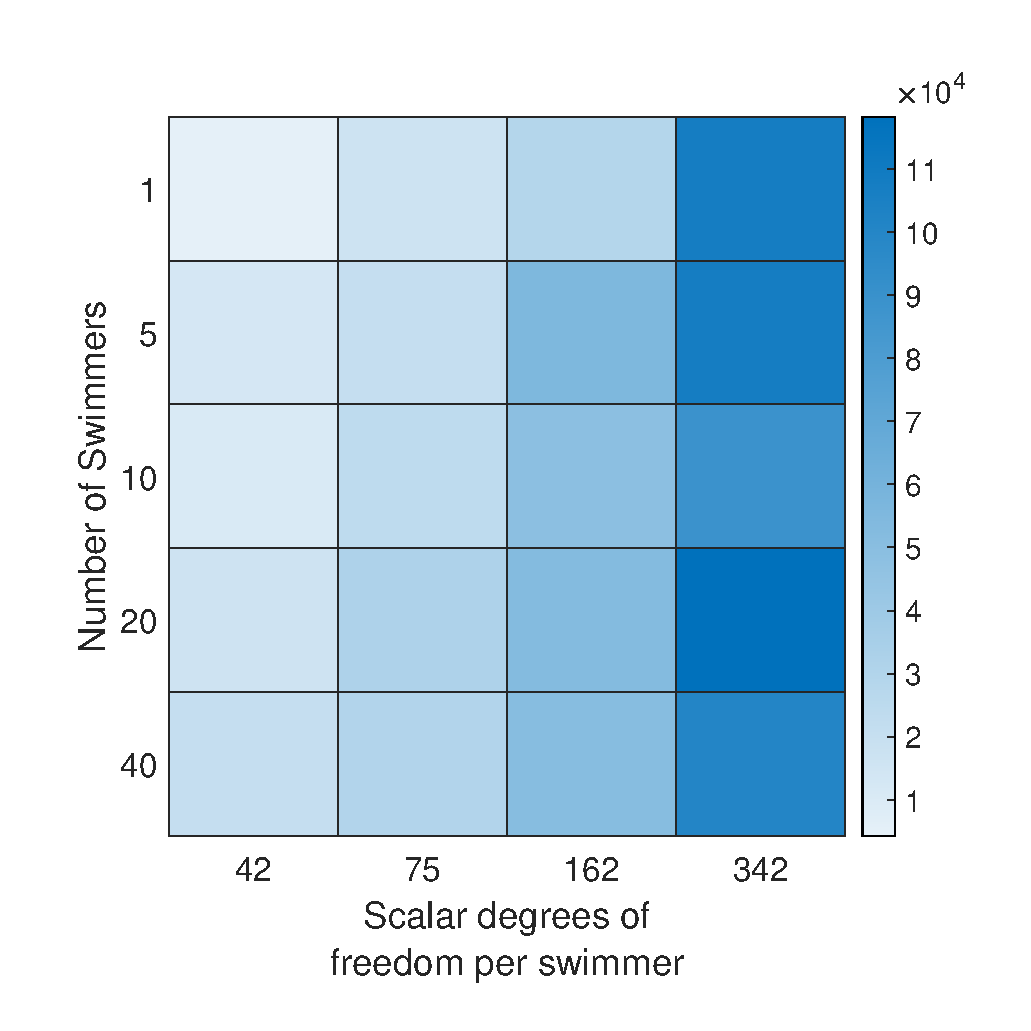
\includegraphics[width=\linewidth]{Images/Condition/Mobility Matrix Preconditioned-1.pdf}
        \caption{Nyström Swimming Matrix with $\epsilon=1e-1$ Preconditioned}
    \end{subfigure}
    \begin{subfigure}{0.3\textwidth}
        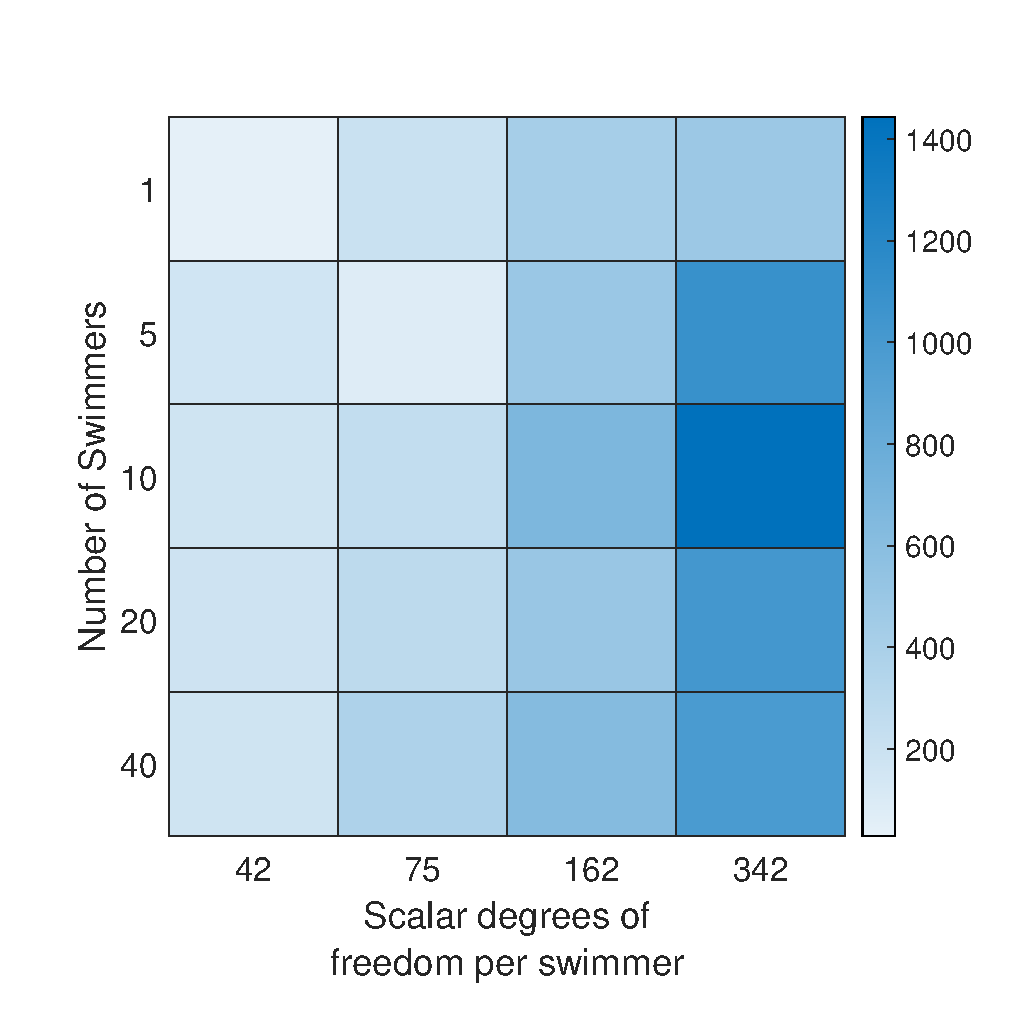
\includegraphics[width=\linewidth]{Images/Condition/Mobility Matrix Preconditioned-2.pdf}
        \caption{Nyström Swimming Matrix with $\epsilon=1e-2$ Preconditioned}
    \end{subfigure}
    \begin{subfigure}{0.3\textwidth}
        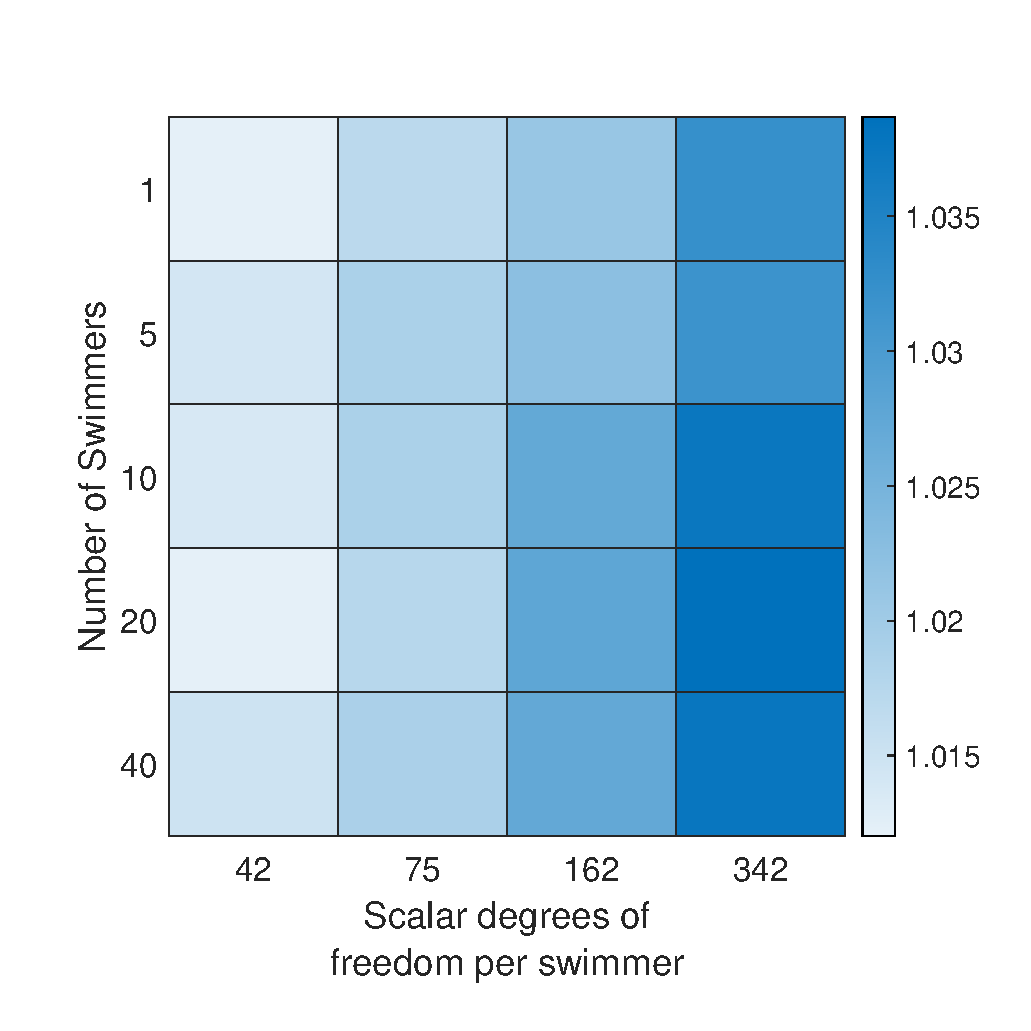
\includegraphics[width=\linewidth]{Images/Condition/Mobility Matrix Preconditioned-5.pdf}
        \caption{Nyström Swimming Matrix with $\epsilon=1e-5$ Preconditioned}
    \end{subfigure}
\end{figure}

\begin{figure}
\ContinuedFloat
    \begin{subfigure}{0.3\textwidth}
        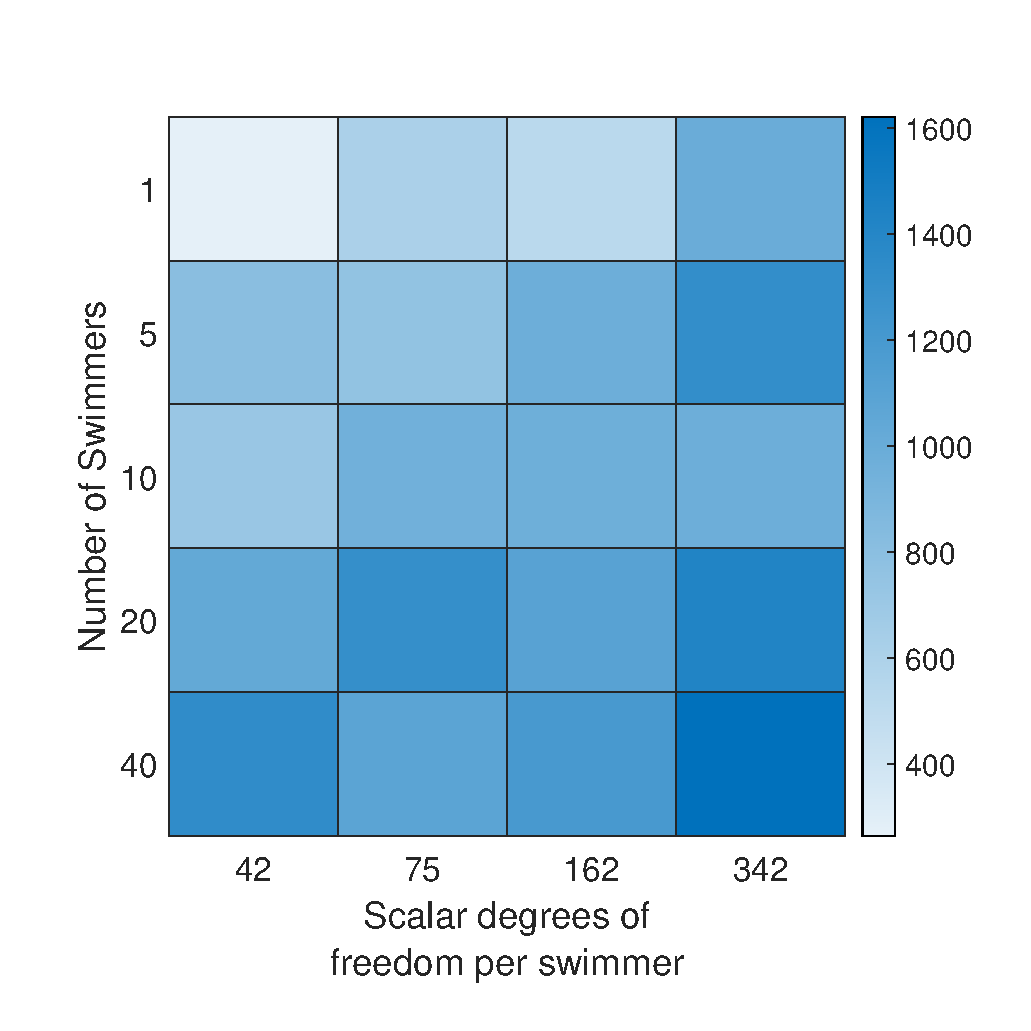
\includegraphics[width=\linewidth]{Images/Condition/Mobility Matrix with rescaled total B Matrix-1.pdf}
        \caption{Nyström Swimming Matrix with $\epsilon=1e-1$ with re-scaled B matrix}
    \end{subfigure}
    \begin{subfigure}{0.3\textwidth}
        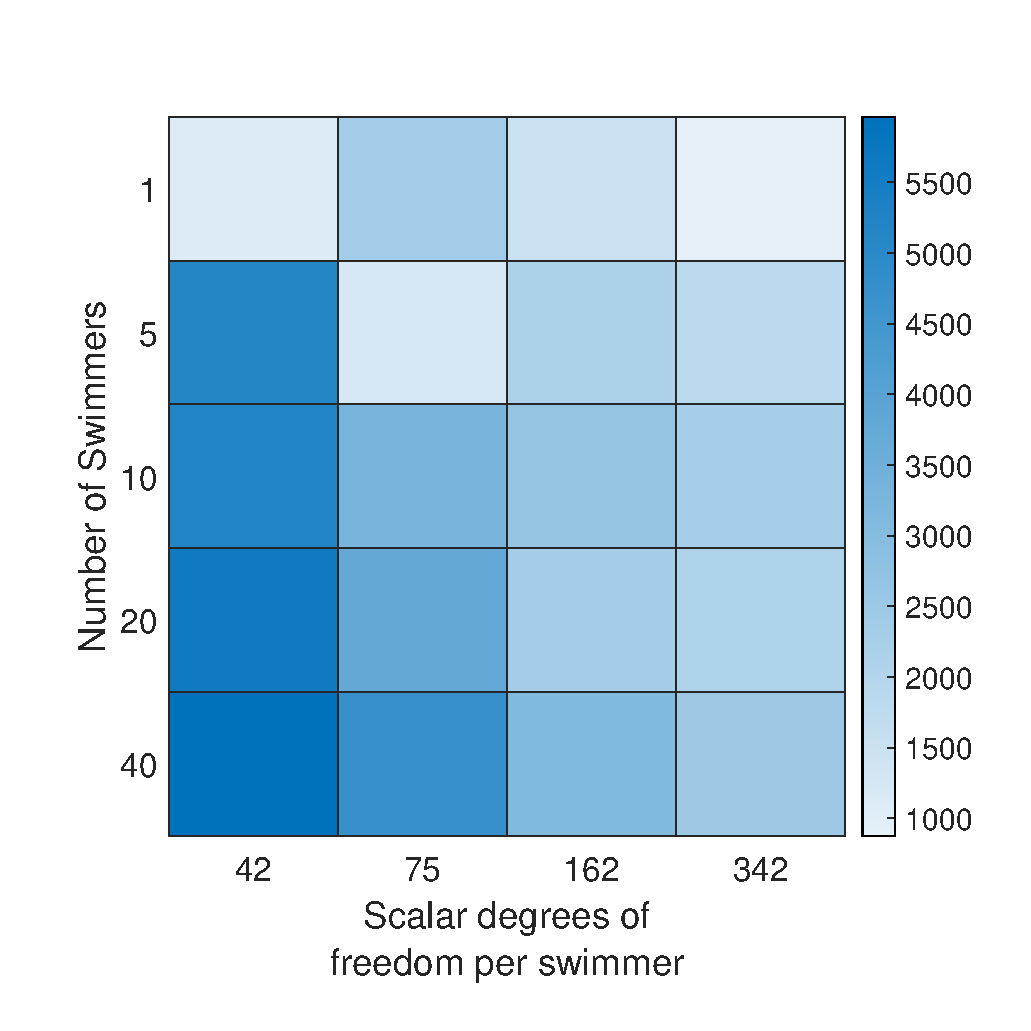
\includegraphics[width=\linewidth]{Images/Condition/Mobility Matrix with rescaled total B Matrix-2.pdf}
        \caption{Nyström Swimming Matrix with $\epsilon=1e-2$ with re-scaled B matrix}
    \end{subfigure}
    \begin{subfigure}{0.3\textwidth}
        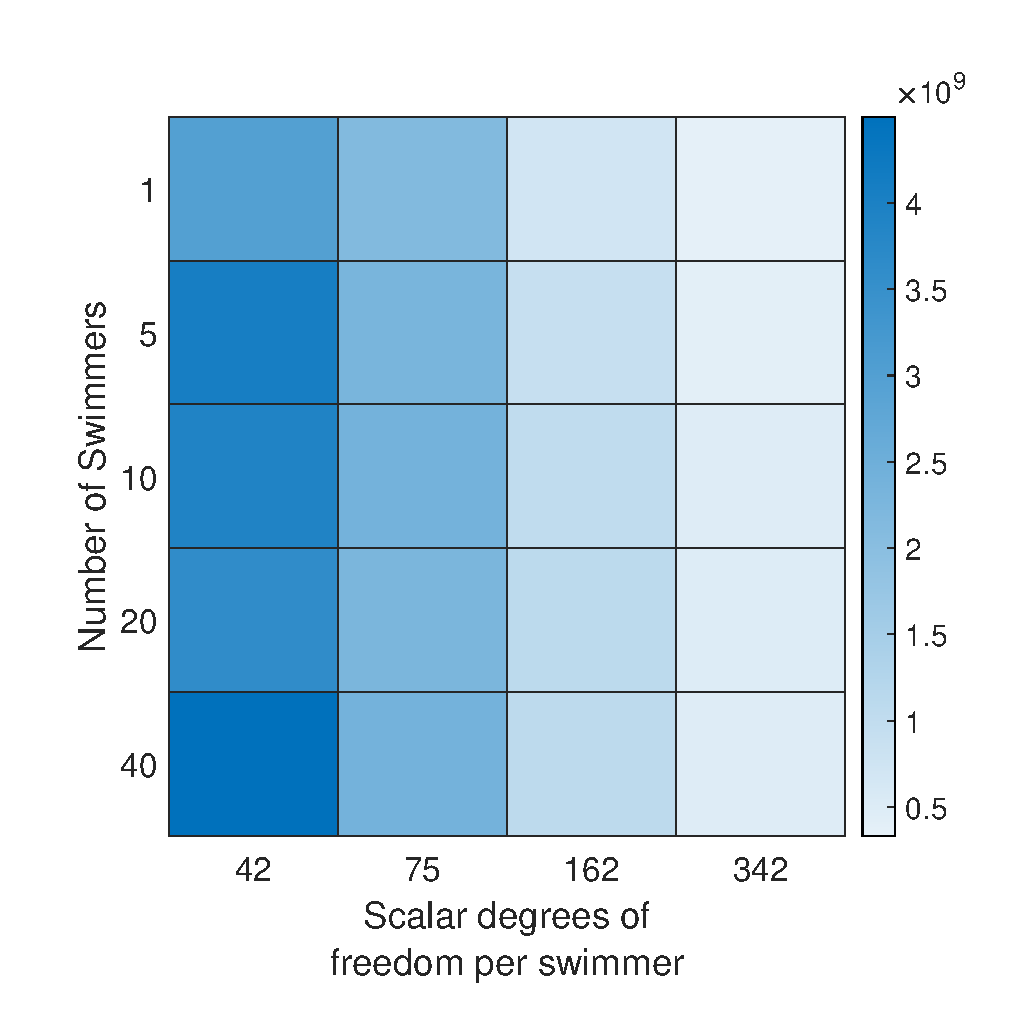
\includegraphics[width=\linewidth]{Images/Condition/Mobility Matrix with rescaled total B Matrix-5.pdf}
        \caption{Nyström Swimming Matrix with $\epsilon=1e-5$ with re-scaled B matrix}
    \end{subfigure}
\end{figure}

\begin{figure}
\ContinuedFloat
    \begin{subfigure}{0.3\textwidth}
        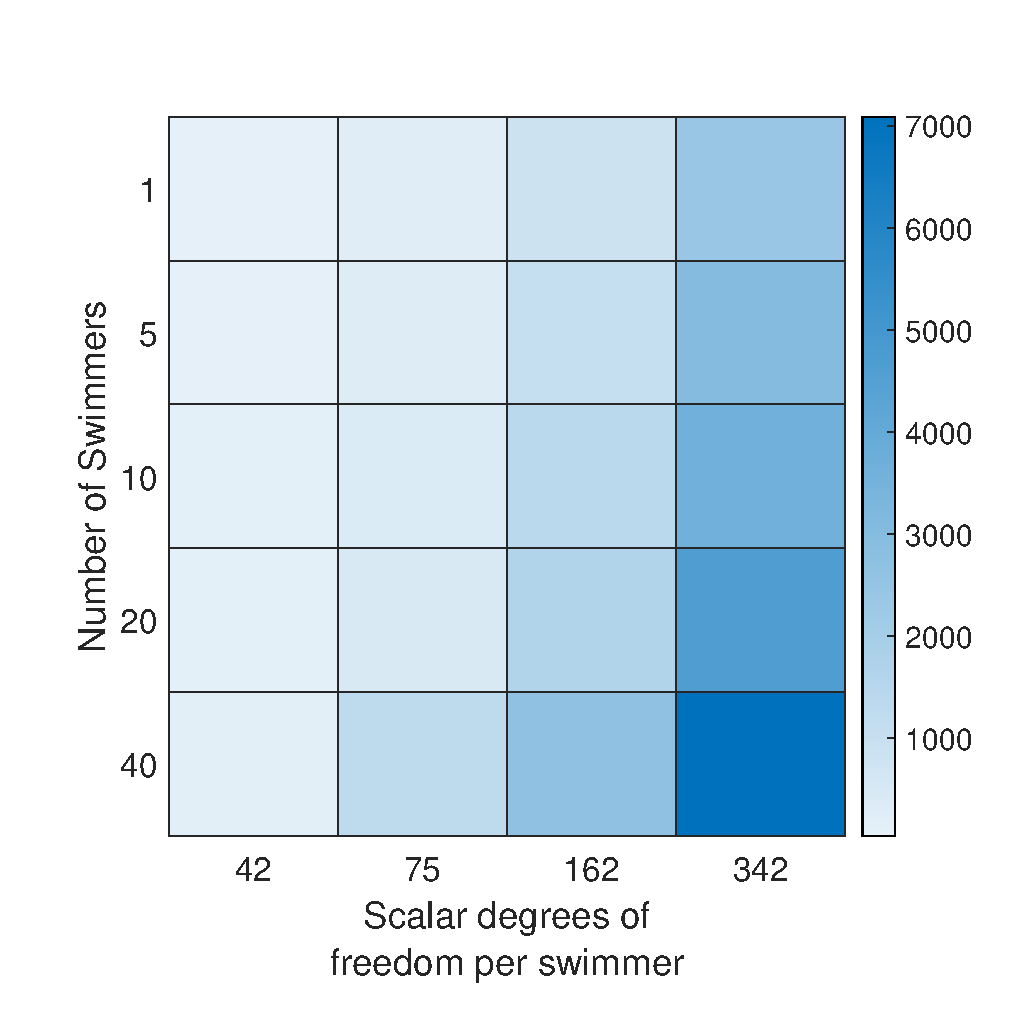
\includegraphics[width=\linewidth]{Images/Condition/Stokeslet Matrix using Disjoint NEAREST-1.pdf}
        \caption{NEAREST Stokeslet Matrix with $\epsilon=1e-1$ with disjoint coarse and fine quadrature sets}
    \end{subfigure}
    \begin{subfigure}{0.3\textwidth}
        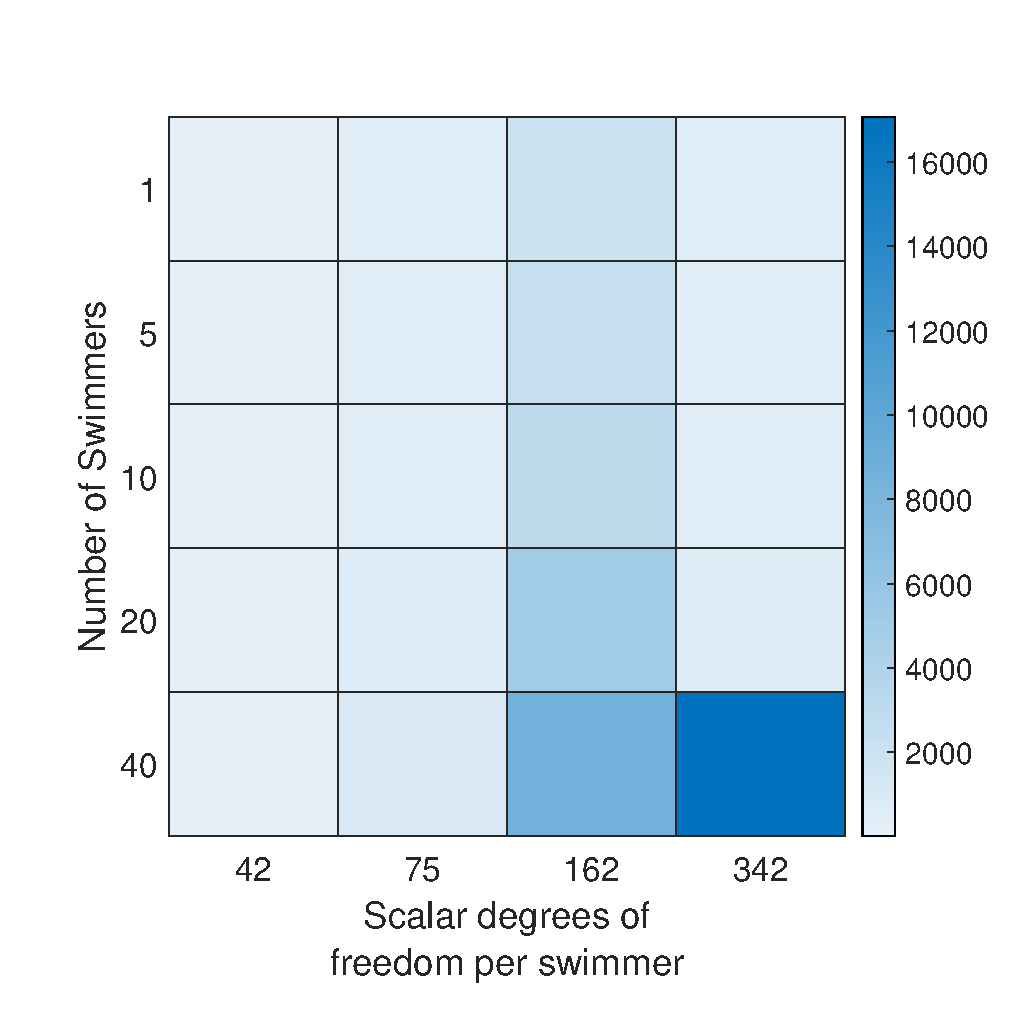
\includegraphics[width=\linewidth]{Images/Condition/Stokeslet Matrix using Disjoint NEAREST-2.pdf}
        \caption{NEAREST Stokeslet Matrix with $\epsilon=1e-2$ with disjoint coarse and fine quadrature sets}
    \end{subfigure}
    \begin{subfigure}{0.3\textwidth}
        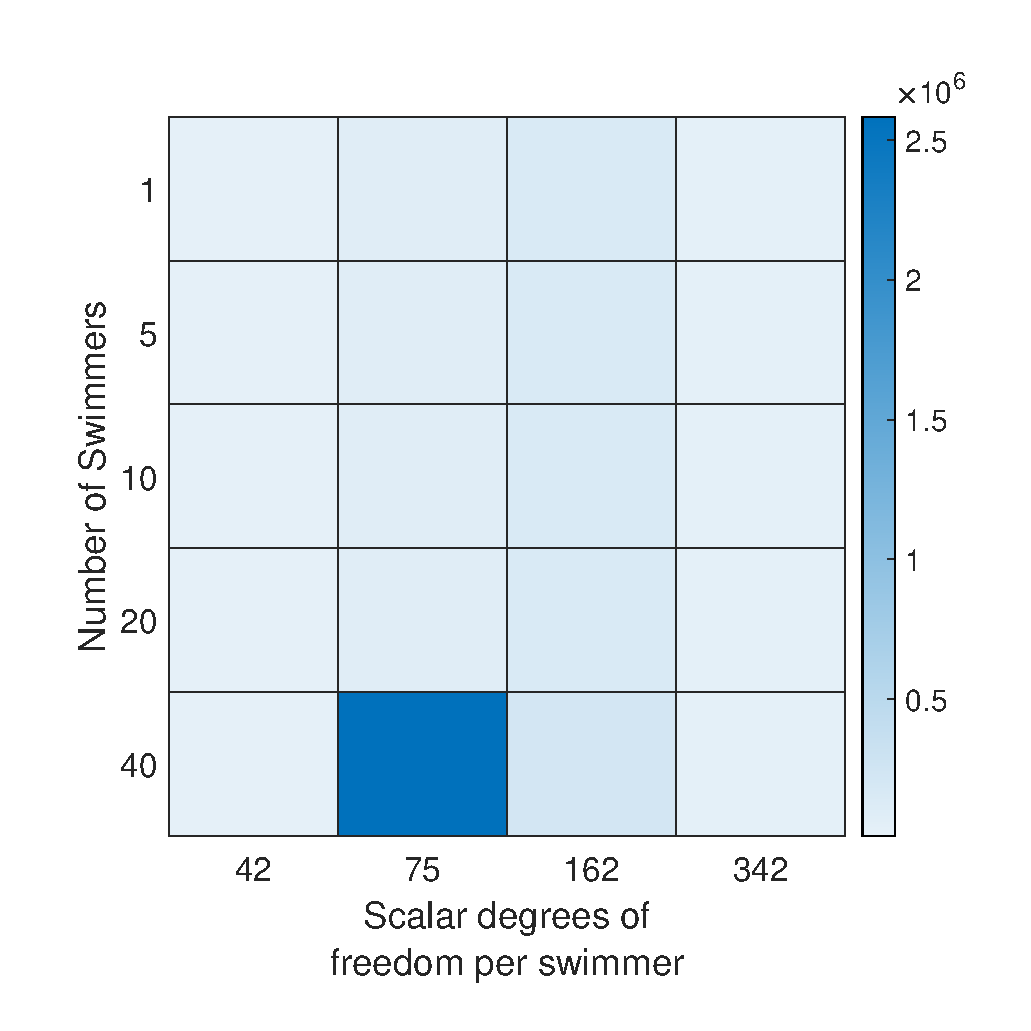
\includegraphics[width=\linewidth]{Images/Condition/Stokeslet Matrix using Disjoint NEAREST-5.pdf}
        \caption{NEAREST Stokeslet Matrix with $\epsilon=1e-5$ with disjoint coarse and fine quadrature sets}
    \end{subfigure}
\end{figure}

\begin{figure}
\ContinuedFloat
    \begin{subfigure}{0.3\textwidth}
        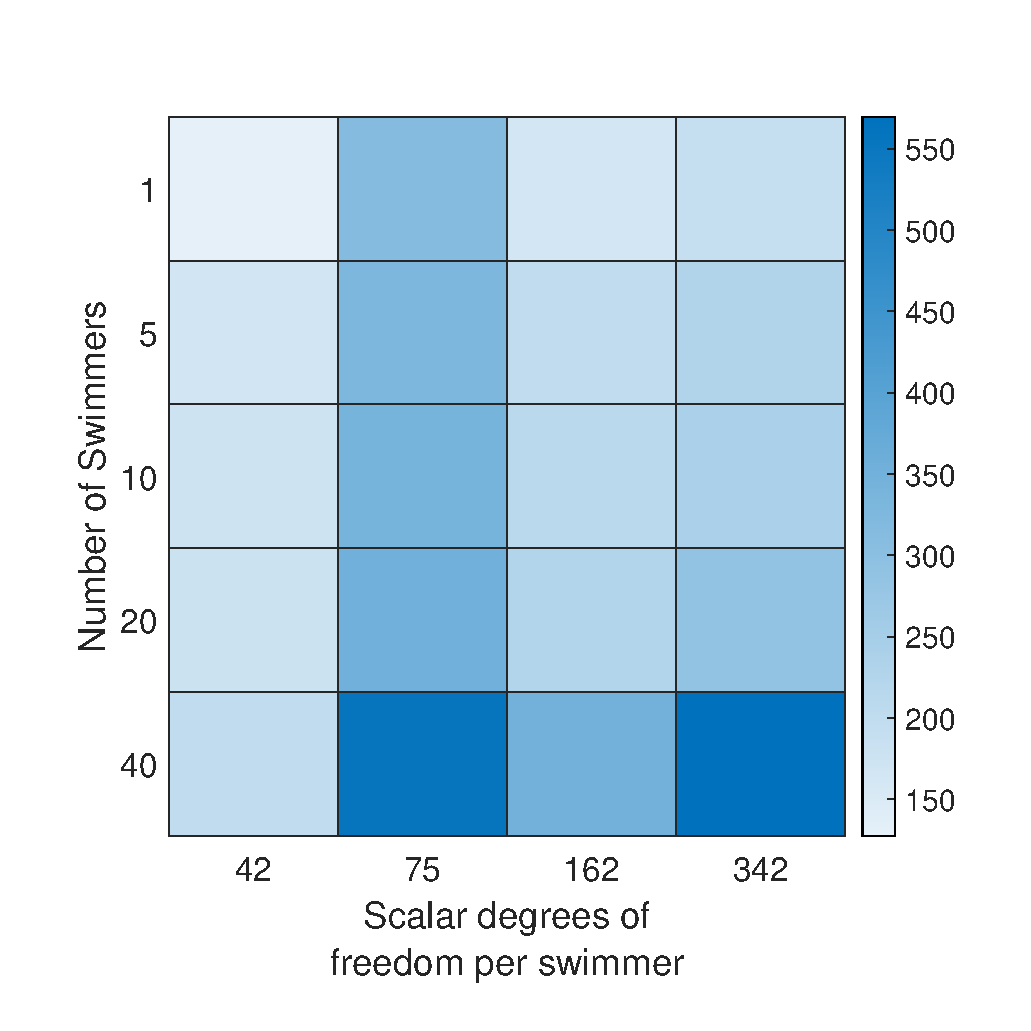
\includegraphics[width=\linewidth]{Images/Condition/Mobility Matrix using Disjoint NEAREST-1.pdf}
        \caption{NEAREST Swimming Matrix with $\epsilon=1e-1$ with disjoint coarse and fine quadrature sets}        
    \end{subfigure}
    \begin{subfigure}{0.3\textwidth}
        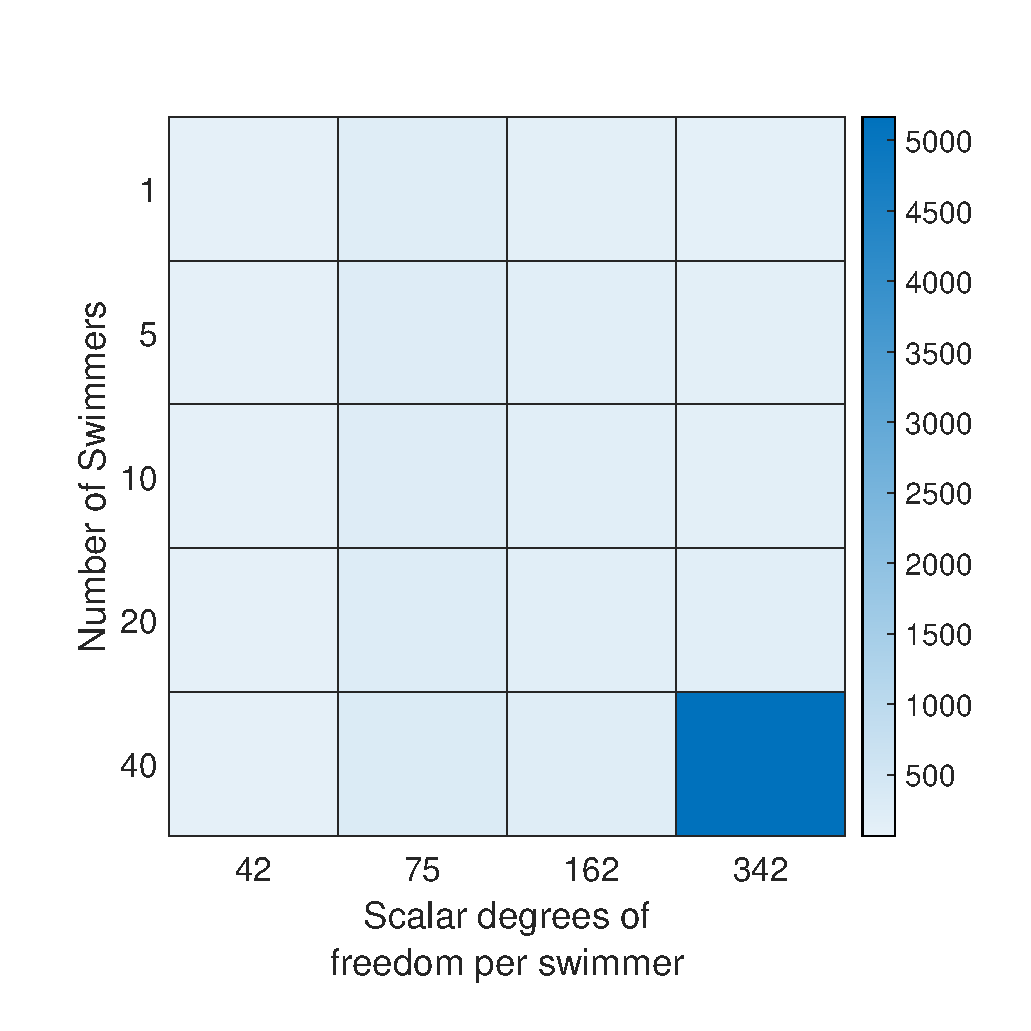
\includegraphics[width=\linewidth]{Images/Condition/Mobility Matrix using Disjoint NEAREST-2.pdf}
        \caption{NEAREST Swimming Matrix with $\epsilon=1e-2$ with disjoint coarse and fine quadrature sets}    
    \end{subfigure}
    \begin{subfigure}{0.3\textwidth}
        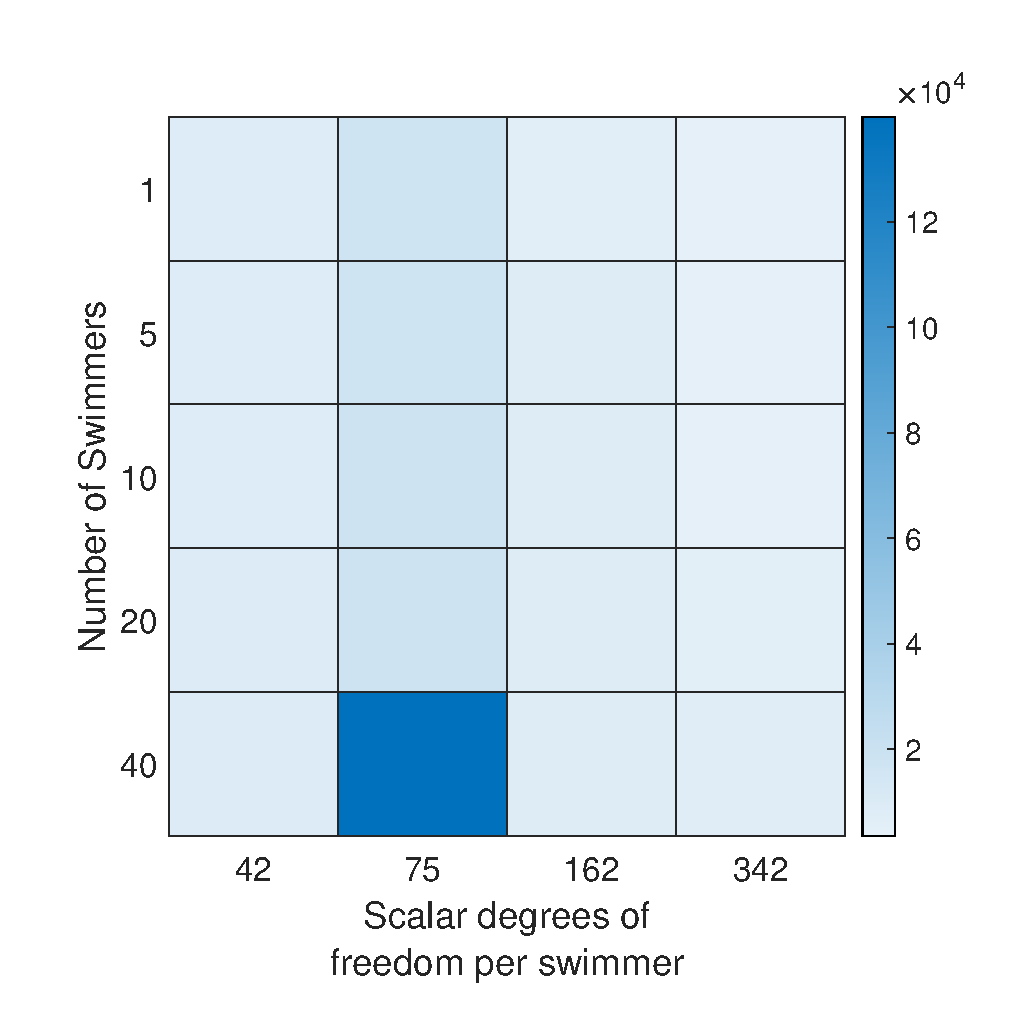
\includegraphics[width=\linewidth]{Images/Condition/Mobility Matrix using Disjoint NEAREST-5.pdf}
        \caption{NEAREST Swimming Matrix with $\epsilon=1e-5$ with disjoint coarse and fine quadrature sets}    
    \end{subfigure}
\end{figure}

\begin{figure}
\ContinuedFloat
    \begin{subfigure}{0.3\textwidth}
        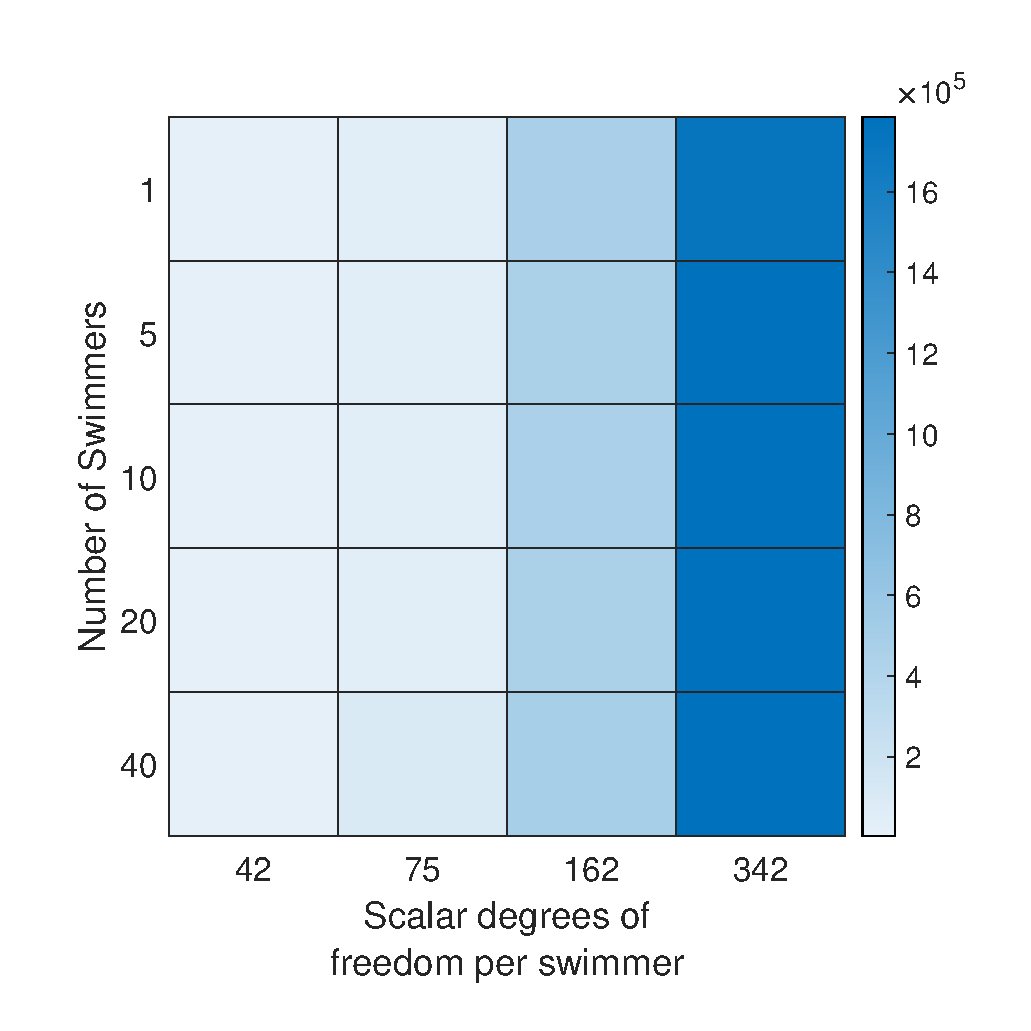
\includegraphics[width=\linewidth]{Images/Condition/Mobility Matrix using Disjoint NEAREST Preconditioned-1.pdf}
        \caption{Preconditioned NEAREST Swimming Matrix with $\epsilon=1e-1$ with disjoint coarse and fine quadrature sets}    
    \end{subfigure}
    \begin{subfigure}{0.3\textwidth}
        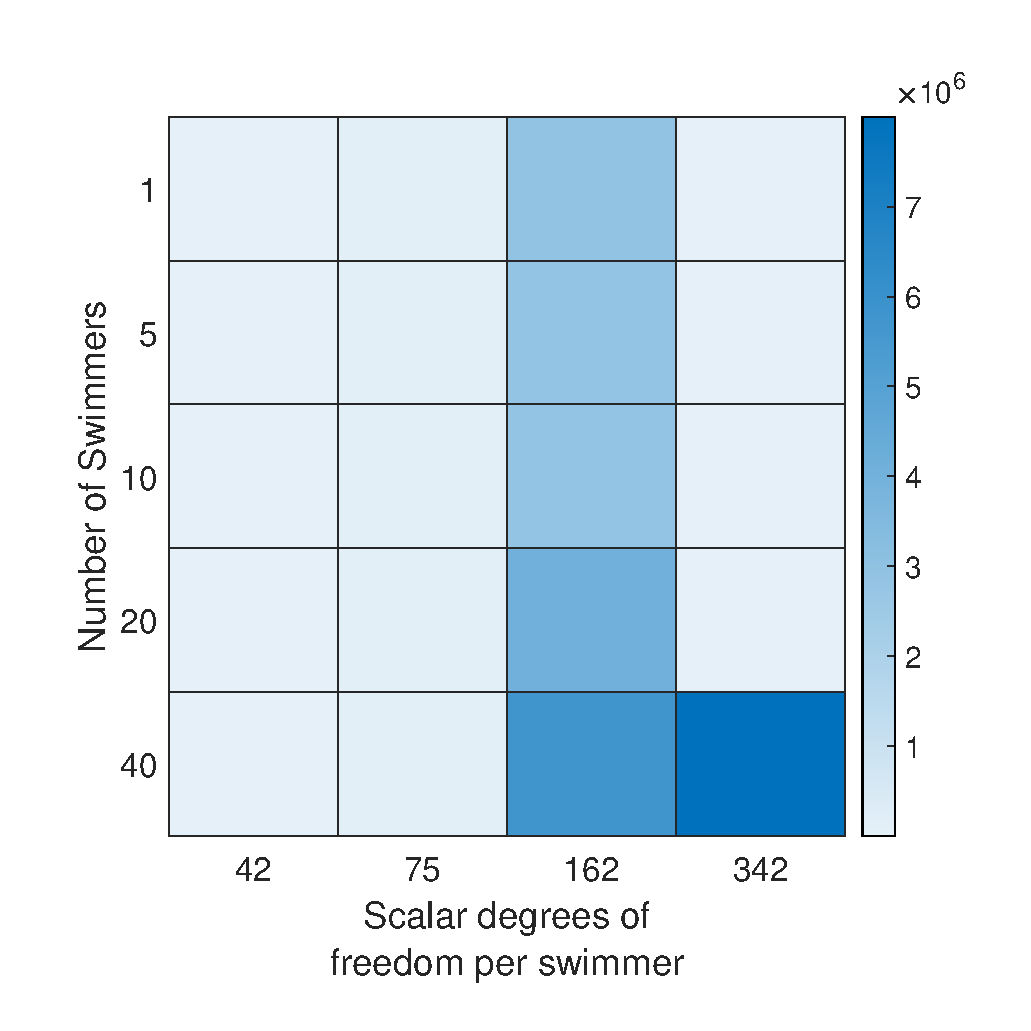
\includegraphics[width=\linewidth]{Images/Condition/Mobility Matrix using Disjoint NEAREST Preconditioned-2.pdf}
        \caption{Preconditioned NEAREST Swimming Matrix with $\epsilon=1e-2$ with disjoint coarse and fine quadrature sets}  
    \end{subfigure}
    \begin{subfigure}{0.3\textwidth}
        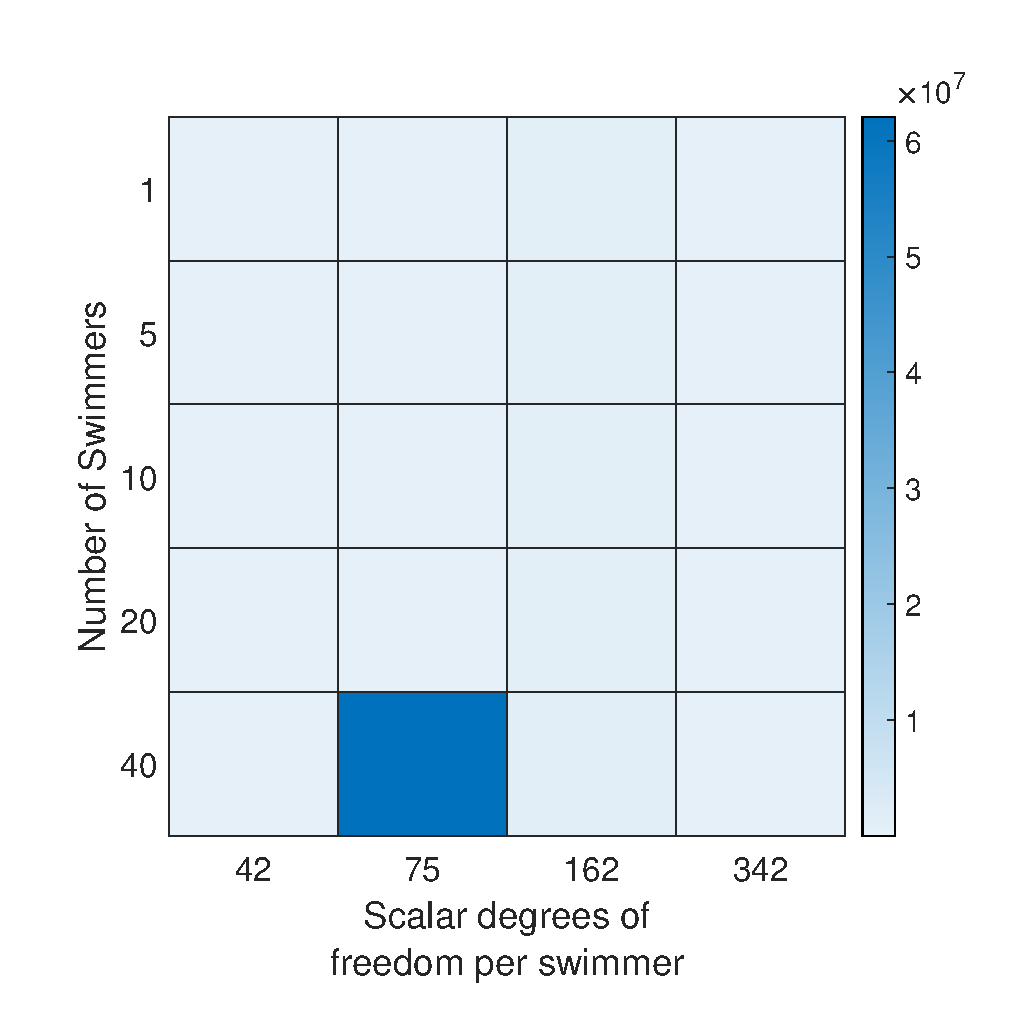
\includegraphics[width=\linewidth]{Images/Condition/Mobility Matrix using Disjoint NEAREST Preconditioned-5.pdf}
        \caption{Preconditioned NEAREST Swimming Matrix with $\epsilon=1e-5$ with disjoint coarse and fine quadrature sets}  
    \end{subfigure}
\end{figure}

\begin{figure}
\ContinuedFloat
    \begin{subfigure}{0.3\textwidth}
        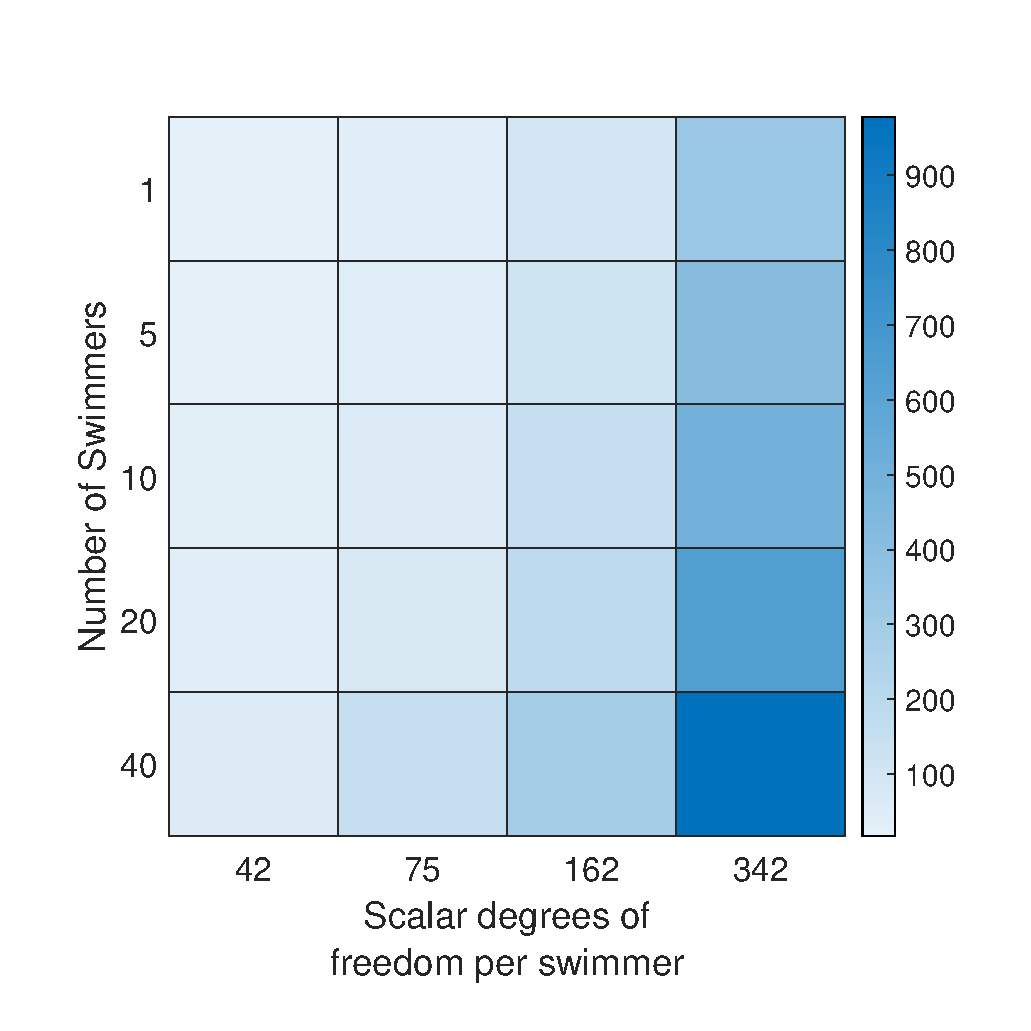
\includegraphics[width=\linewidth]{Images/Condition/Stokeslet Matrix using Contained NEAREST-1.pdf}
        \caption{NEAREST Stokeslet Matrix with $\epsilon=1e-1$ with joint coarse and fine quadrature sets}
    \end{subfigure}
    \begin{subfigure}{0.3\textwidth}
        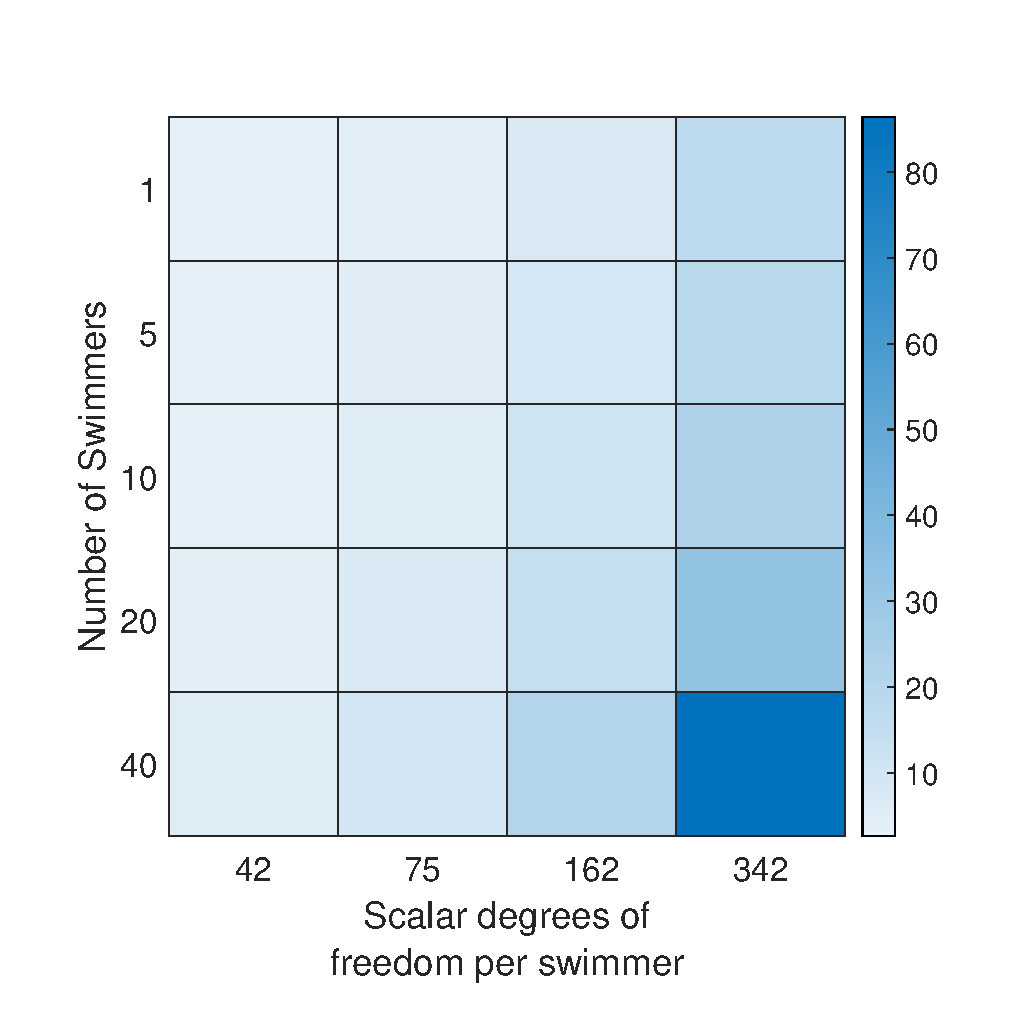
\includegraphics[width=\linewidth]{Images/Condition/Stokeslet Matrix using Contained NEAREST-2.pdf}
        \caption{NEAREST Stokeslet Matrix with $\epsilon=1e-2$ with joint coarse and fine quadrature sets}
    \end{subfigure}
    \begin{subfigure}{0.3\textwidth}
        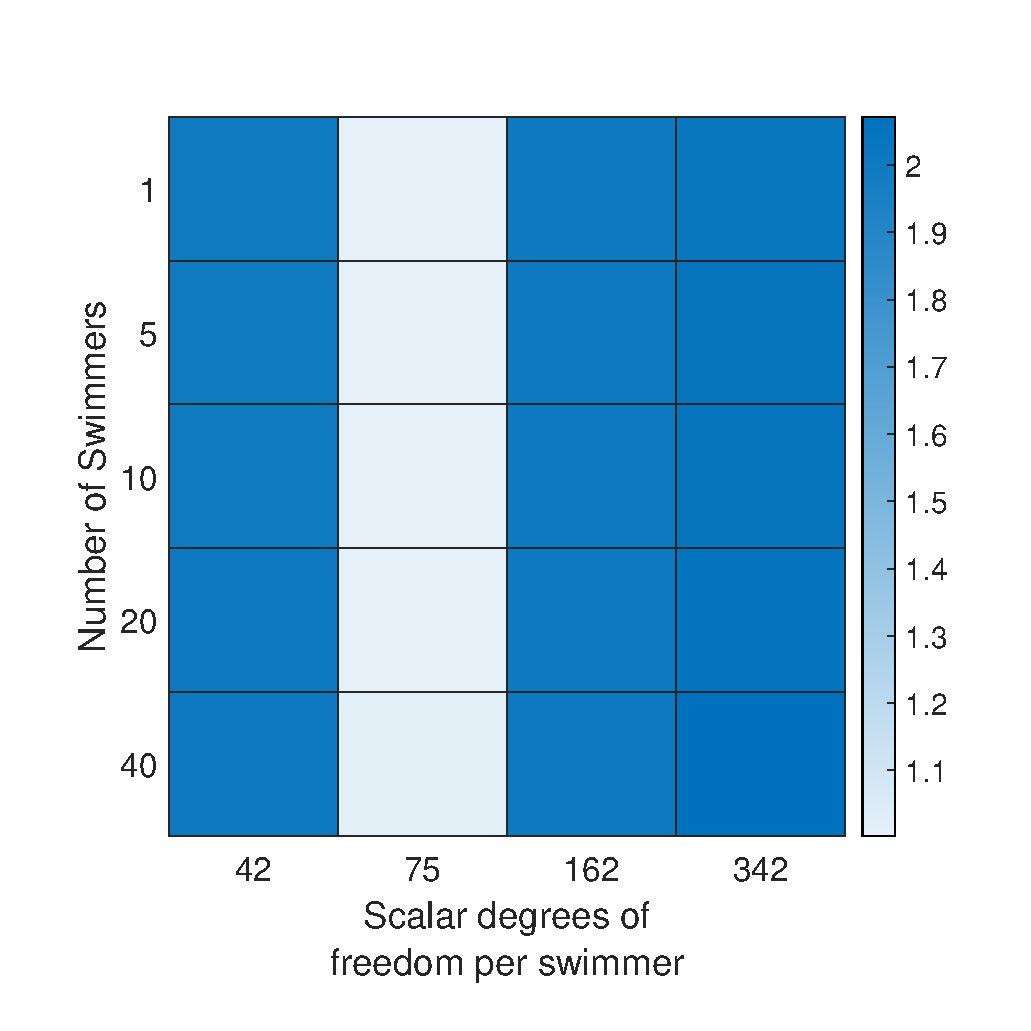
\includegraphics[width=\linewidth]{Images/Condition/Stokeslet Matrix using Contained NEAREST-5.pdf}
        \caption{NEAREST Stokeslet Matrix with $\epsilon=1e-5$ with joint coarse and fine quadrature sets}
    \end{subfigure}
\end{figure}

\begin{figure}
\ContinuedFloat
    \begin{subfigure}{0.3\textwidth}
        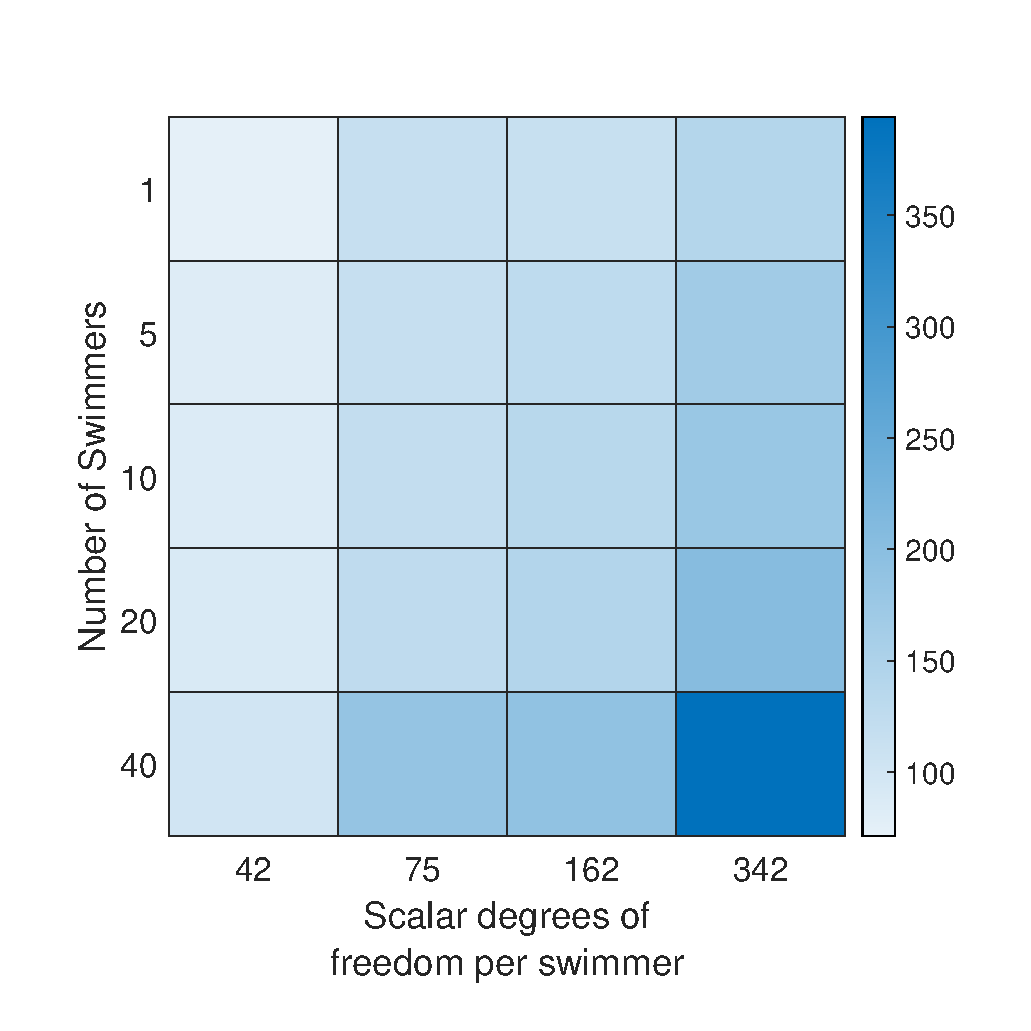
\includegraphics[width=\linewidth]{Images/Condition/Mobility Matrix using Contained NEAREST-1.pdf}
        \caption{NEAREST Swimming Matrix with $\epsilon=1e-1$ with joint coarse and fine quadrature sets}        
    \end{subfigure}
    \begin{subfigure}{0.3\textwidth}
        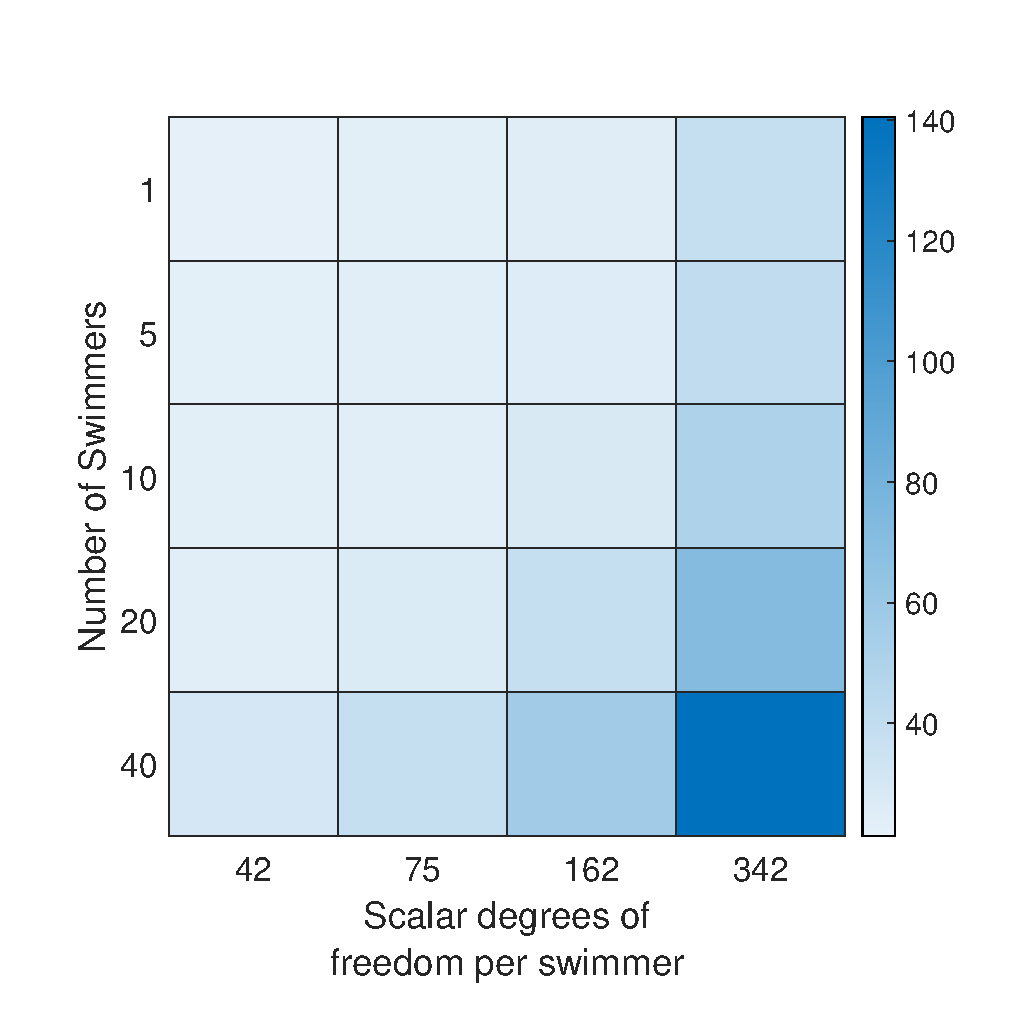
\includegraphics[width=\linewidth]{Images/Condition/Mobility Matrix using Contained NEAREST-2.pdf}
        \caption{NEAREST Swimming Matrix with $\epsilon=1e-2$ with joint coarse and fine quadrature sets}    
    \end{subfigure}
    \begin{subfigure}{0.3\textwidth}
        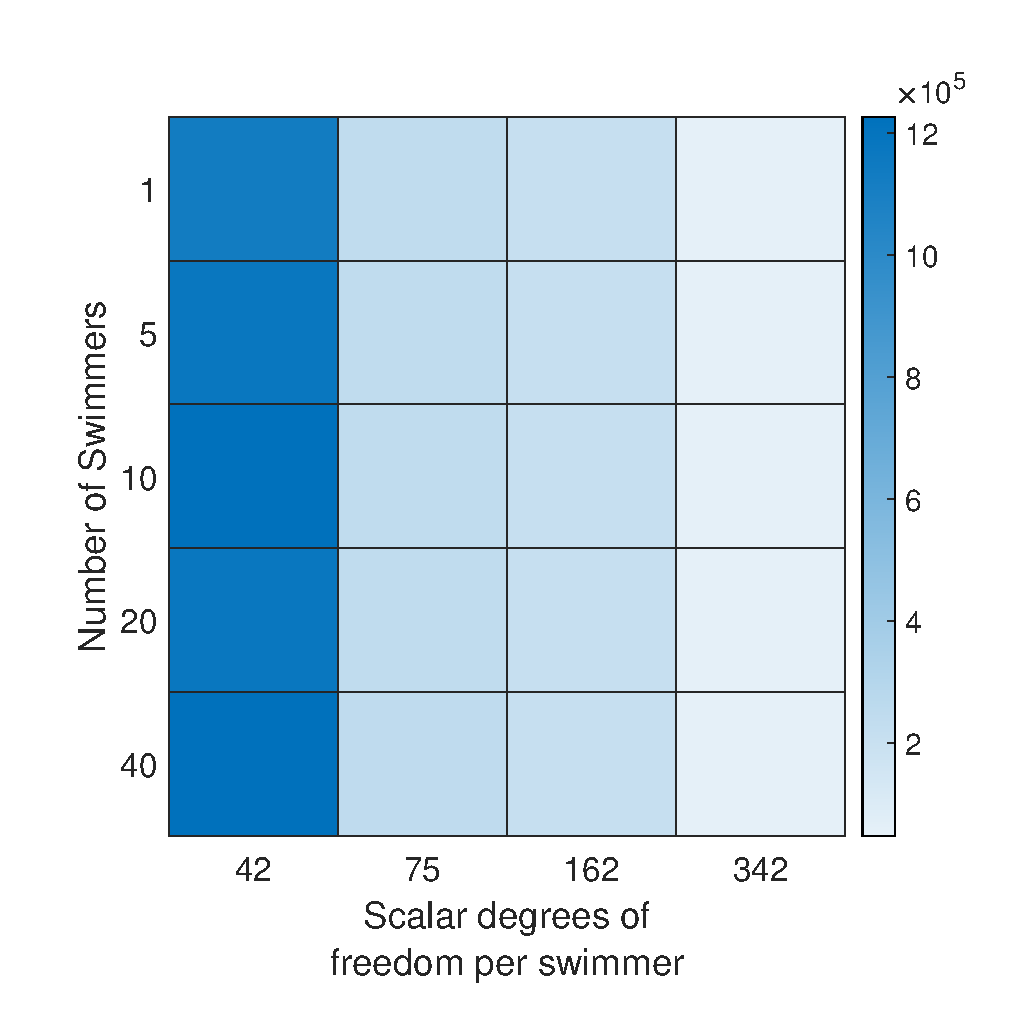
\includegraphics[width=\linewidth]{Images/Condition/Mobility Matrix using Contained NEAREST-5.pdf}
        \caption{NEAREST Swimming Matrix with $\epsilon=1e-5$ with joint coarse and fine quadrature sets}    
    \end{subfigure}
\end{figure}

\begin{figure}
\ContinuedFloat
    \begin{subfigure}{0.3\textwidth}
        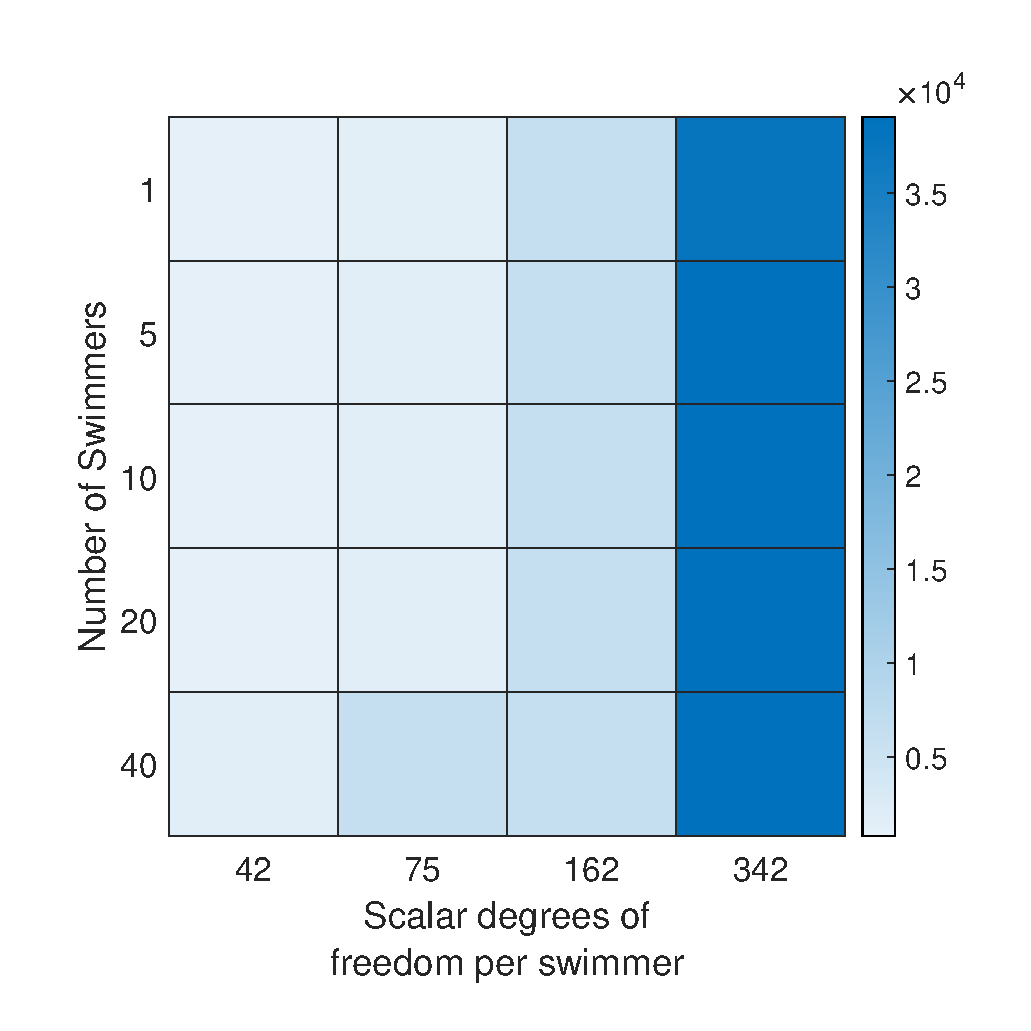
\includegraphics[width=\linewidth]{Images/Condition/Mobility Matrix using Contained NEAREST Preconditioned-1.pdf}
        \caption{Preconditioned NEAREST Swimming Matrix with $\epsilon=1e-1$ with joint coarse and fine quadrature sets}    
    \end{subfigure}
    \begin{subfigure}{0.3\textwidth}
        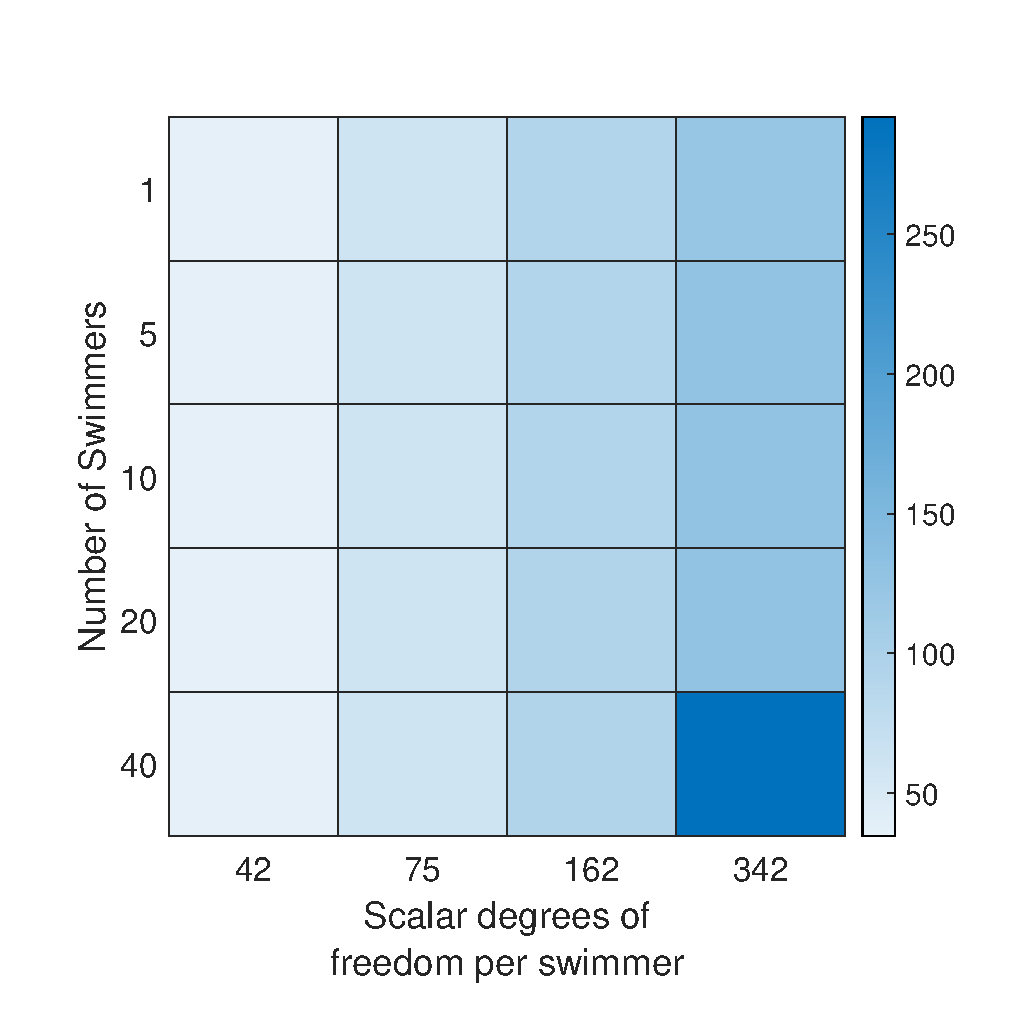
\includegraphics[width=\linewidth]{Images/Condition/Mobility Matrix using Contained NEAREST Preconditioned-2.pdf}
        \caption{Preconditioned NEAREST Swimming Matrix with $\epsilon=1e-2$ with joint coarse and fine quadrature sets}  
    \end{subfigure}
    \begin{subfigure}{0.3\textwidth}
        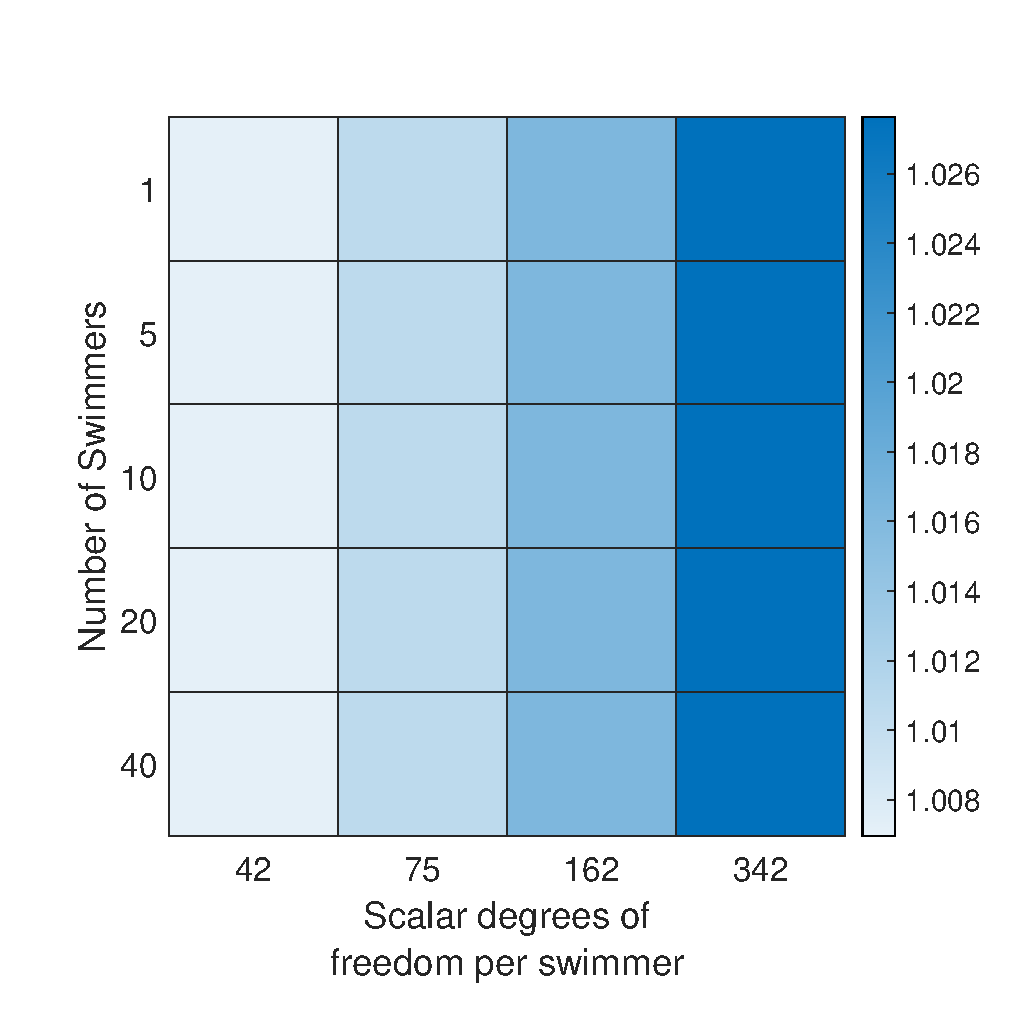
\includegraphics[width=\linewidth]{Images/Condition/Mobility Matrix using Contained NEAREST Preconditioned-5.pdf}
        \caption{Preconditioned NEAREST Swimming Matrix with $\epsilon=1e-5$ with joint coarse and fine quadrature sets}  
    \end{subfigure}
\end{figure}

\begin{figure}
\caption[Eigenvalues of matrices considered in this paper.]{Eigenvalues of matrices considered in this paper for the case of 40 swimmers and 114 force quadrature points.}
    \begin{subfigure}{0.45\textwidth}
        \centering
        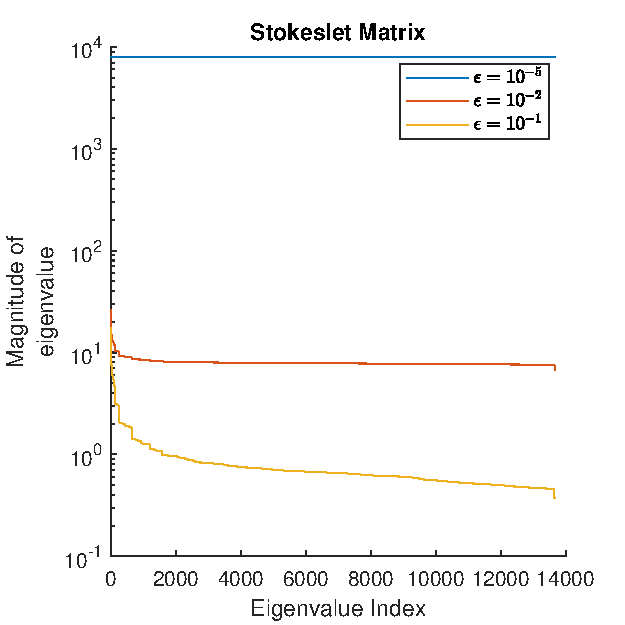
\includegraphics[width=\linewidth]{Images/Condition/Eigen-Stokeslet Matrix.pdf}
    \end{subfigure}
    \hfill
    \begin{subfigure}{0.45\textwidth}
        \centering
        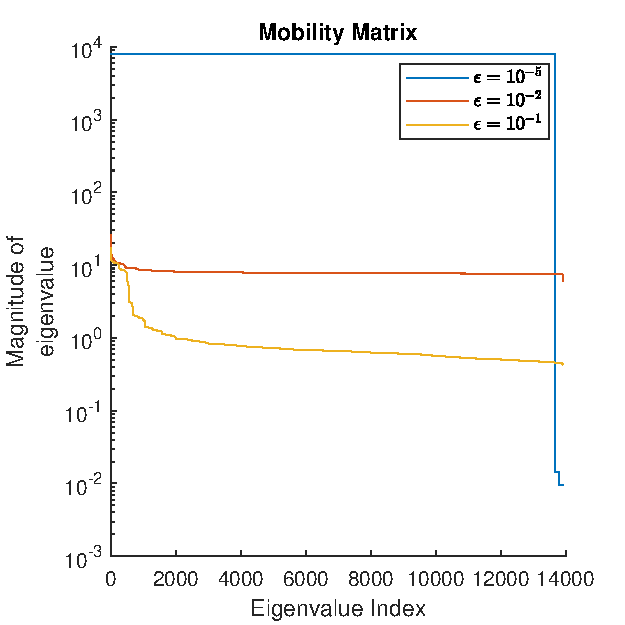
\includegraphics[width=\linewidth]{Images/Condition/Eigen-Mobility Matrix.pdf}
    \end{subfigure}
\end{figure}
\begin{figure}
\ContinuedFloat
    \begin{subfigure}{0.45\textwidth}
        \centering
        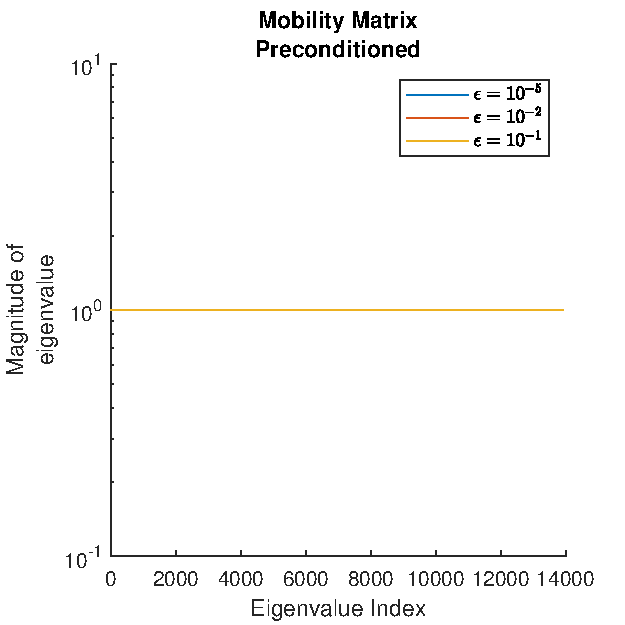
\includegraphics[width=\linewidth]{Images/Condition/Eigen-Mobility Matrix Preconditioned.pdf}
    \end{subfigure}
    \hfill
    \begin{subfigure}{0.45\textwidth}
        \centering
        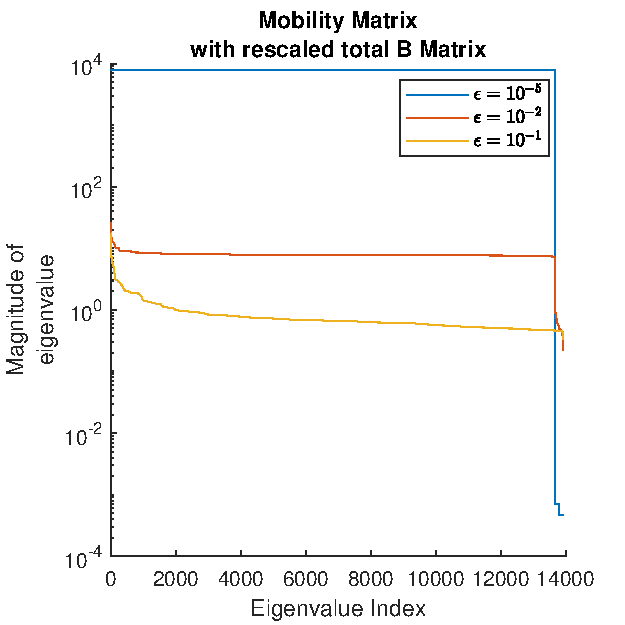
\includegraphics[width=\linewidth]{Images/Condition/Eigen-Mobility Matrix with rescaled total B Matrix.pdf}
    \end{subfigure}
\end{figure}
\begin{figure}
\ContinuedFloat
    \begin{subfigure}{0.45\textwidth}
        \centering
        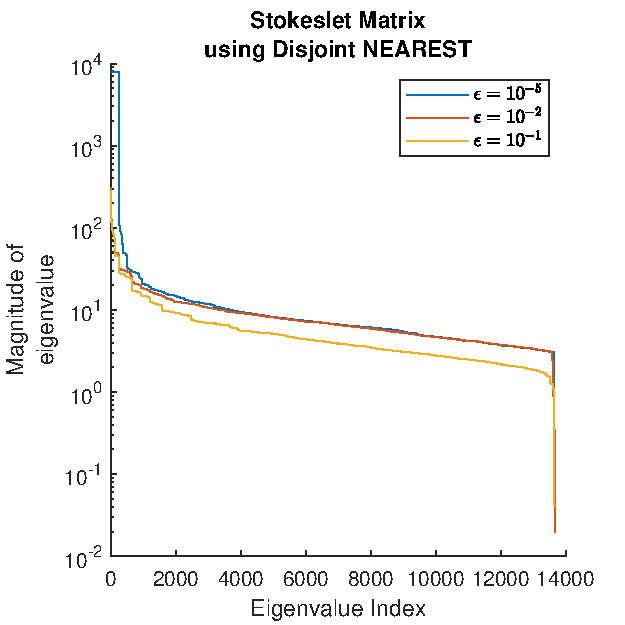
\includegraphics[width=\linewidth]{Images/Condition/Eigen-Stokeslet Matrix using Disjoint NEAREST.pdf}
    \end{subfigure}
    \hfill
    \begin{subfigure}{0.45\textwidth}
        \centering
        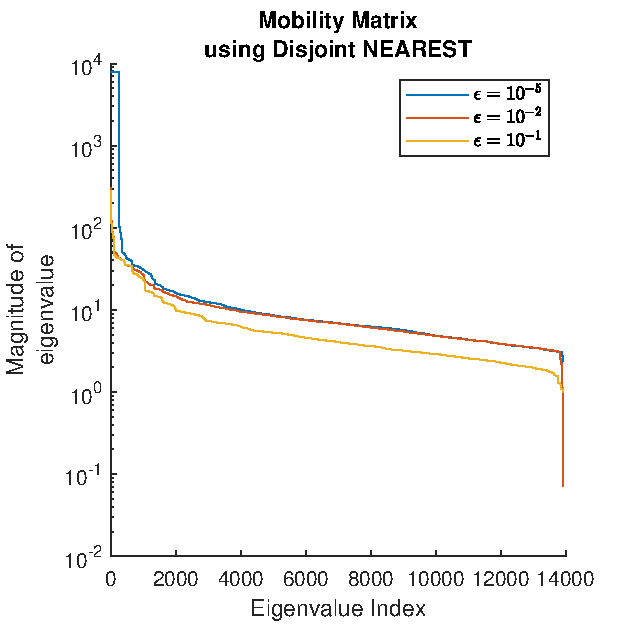
\includegraphics[width=\linewidth]{Images/Condition/Eigen-Mobility Matrix using Disjoint NEAREST.pdf}
    \end{subfigure}
\end{figure}

\begin{figure}
\ContinuedFloat
    \begin{subfigure}{0.45\textwidth}
        \centering
        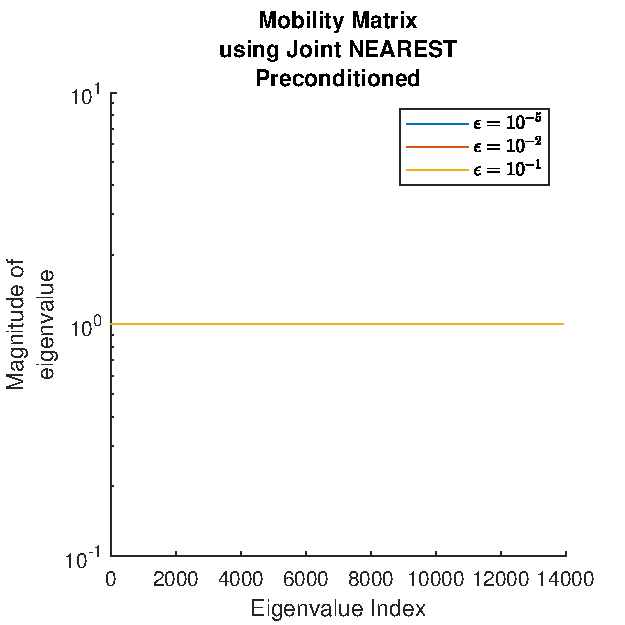
\includegraphics[width=\linewidth]{Images/Condition/Eigen-Mobility Matrix using Joint NEAREST Preconditioned.pdf}
    \end{subfigure}
    \hfill
    \begin{subfigure}{0.45\textwidth}
        \centering
        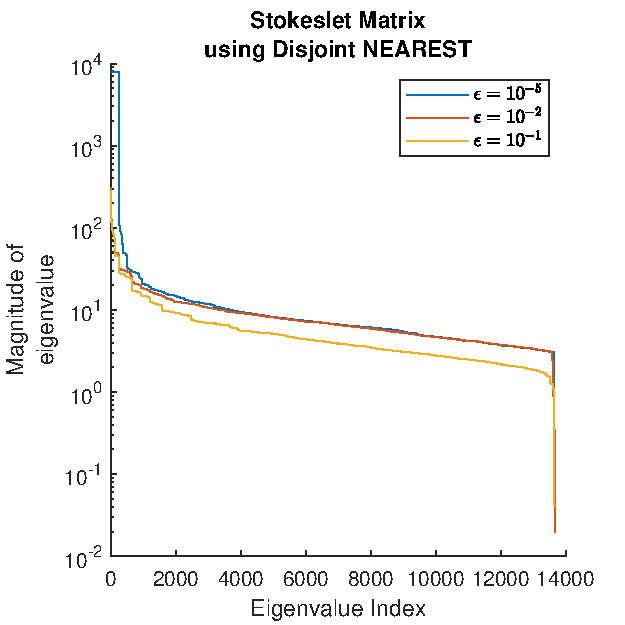
\includegraphics[width=\linewidth]{Images/Condition/Eigen-Stokeslet Matrix using Disjoint NEAREST.pdf}
    \end{subfigure}
\end{figure}
\begin{figure}
\ContinuedFloat
    \begin{subfigure}{0.45\textwidth}
        \centering
        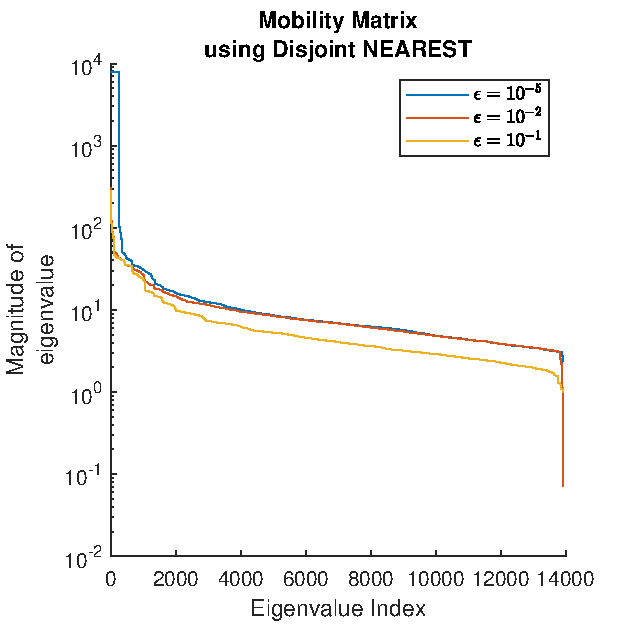
\includegraphics[width=\linewidth]{Images/Condition/Eigen-Mobility Matrix using Disjoint NEAREST.pdf}
    \end{subfigure}
    \hfill
    \begin{subfigure}{0.45\textwidth}
        \centering
        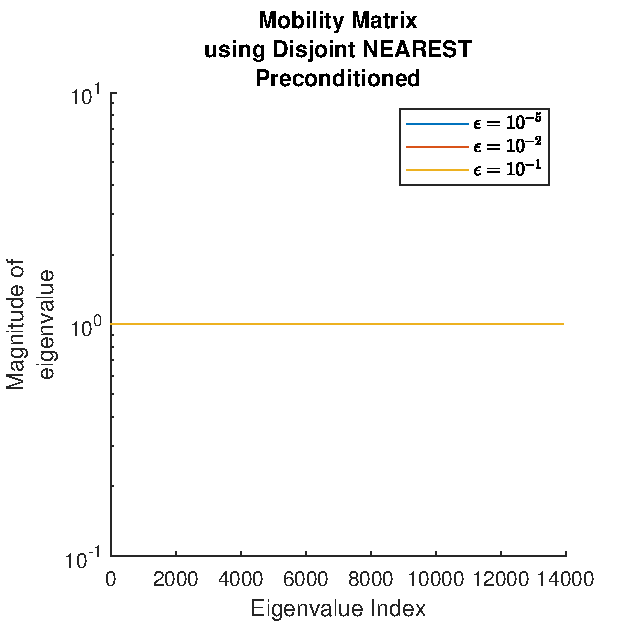
\includegraphics[width=\linewidth]{Images/Condition/Eigen-Mobility Matrix using Disjoint NEAREST Preconditioned.pdf}
    \end{subfigure}
\end{figure}



\begin{comment}
 \begin{sidewaysfigure}[!ht]
     \centering
     \begin{subfigure}[b]{0.49\textwidth}
         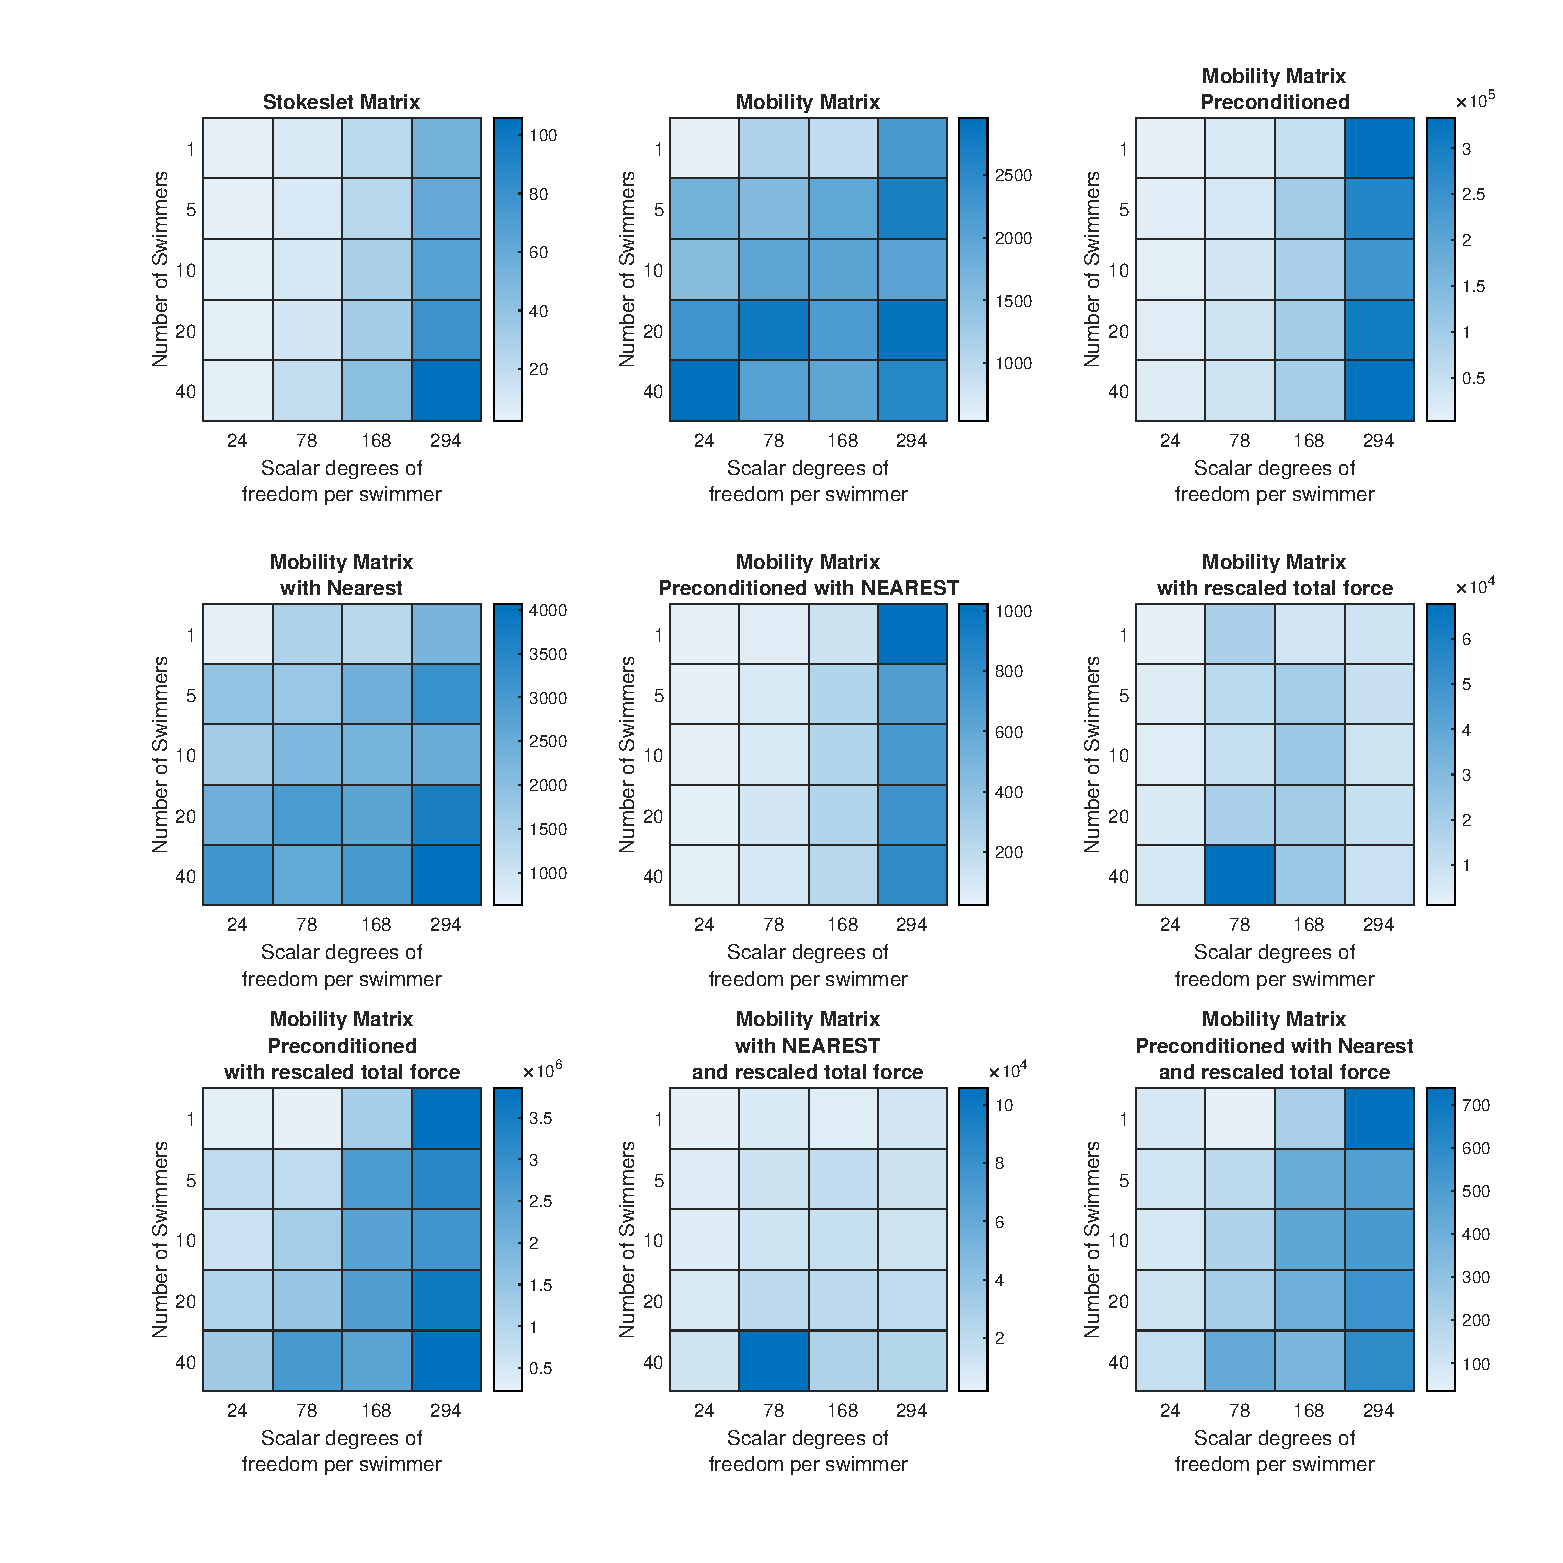
\includegraphics[height=0.49\textheight,keepaspectratio]{Images/Condition/Condition-1.pdf}
         \caption{Figure showing the condition number for various matrices shown in the paper for the case of $\epsilon=1e-1$.}
         \label{fig:Condition1}
     \end{subfigure}
     \hfill
     \begin{subfigure}[b]{0.49\textheight}
         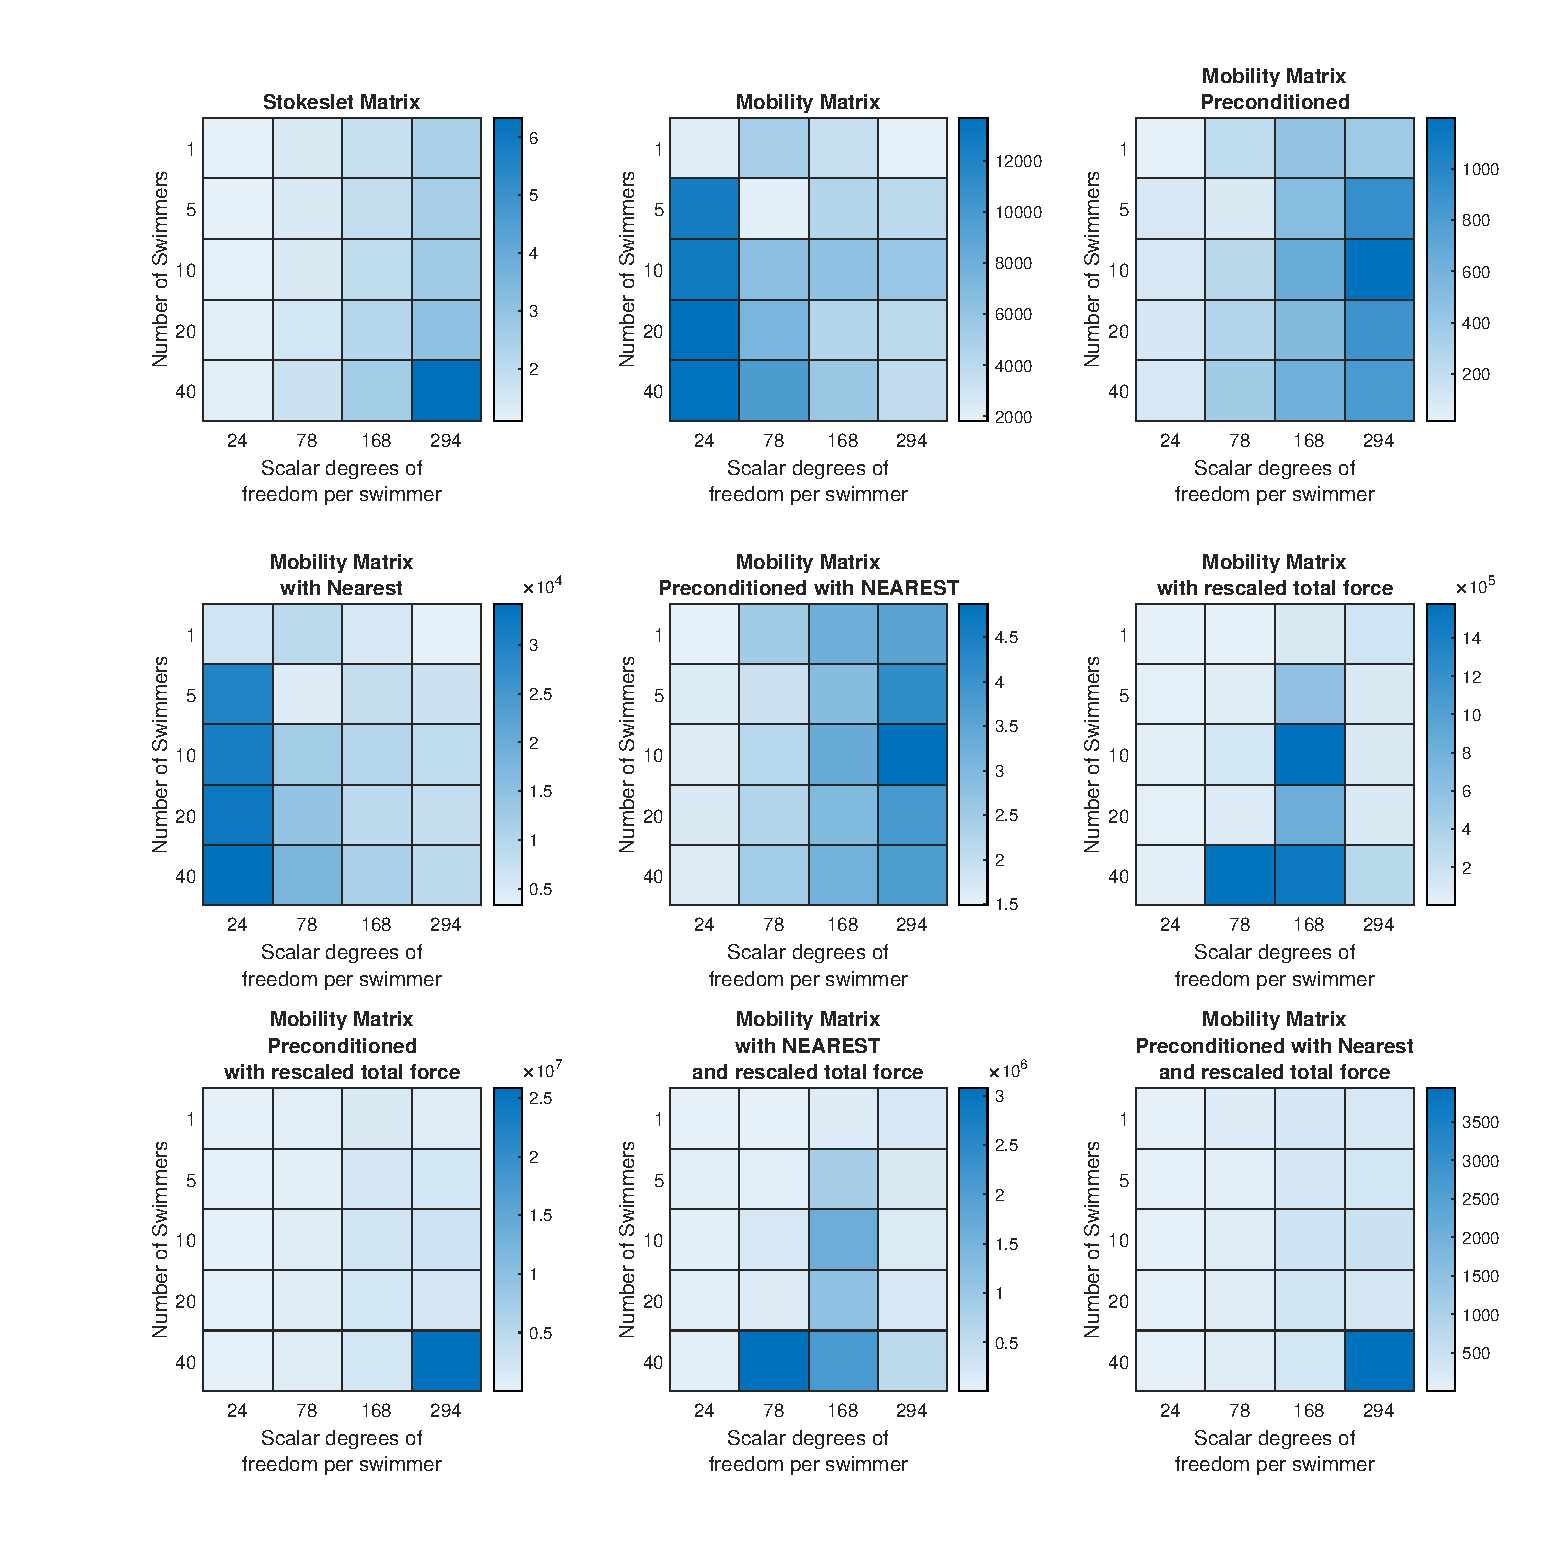
\includegraphics[height=0.49\textheight,keepaspectratio]{Images/Condition/Condition-2.pdf}
         \caption{Figure showing the condition number for various matrices shown in the paper for the case of $\epsilon=1e-2$.}
         \label{fig:Condition2}
     \end{subfigure}
\end{sidewaysfigure}
\begin{sidewaysfigure}[!htbp]
\ContinuedFloat
     \centering
     \begin{subfigure}[b]{0.49\textheight}
        \captionsetup{width=0.49\textwidth}
        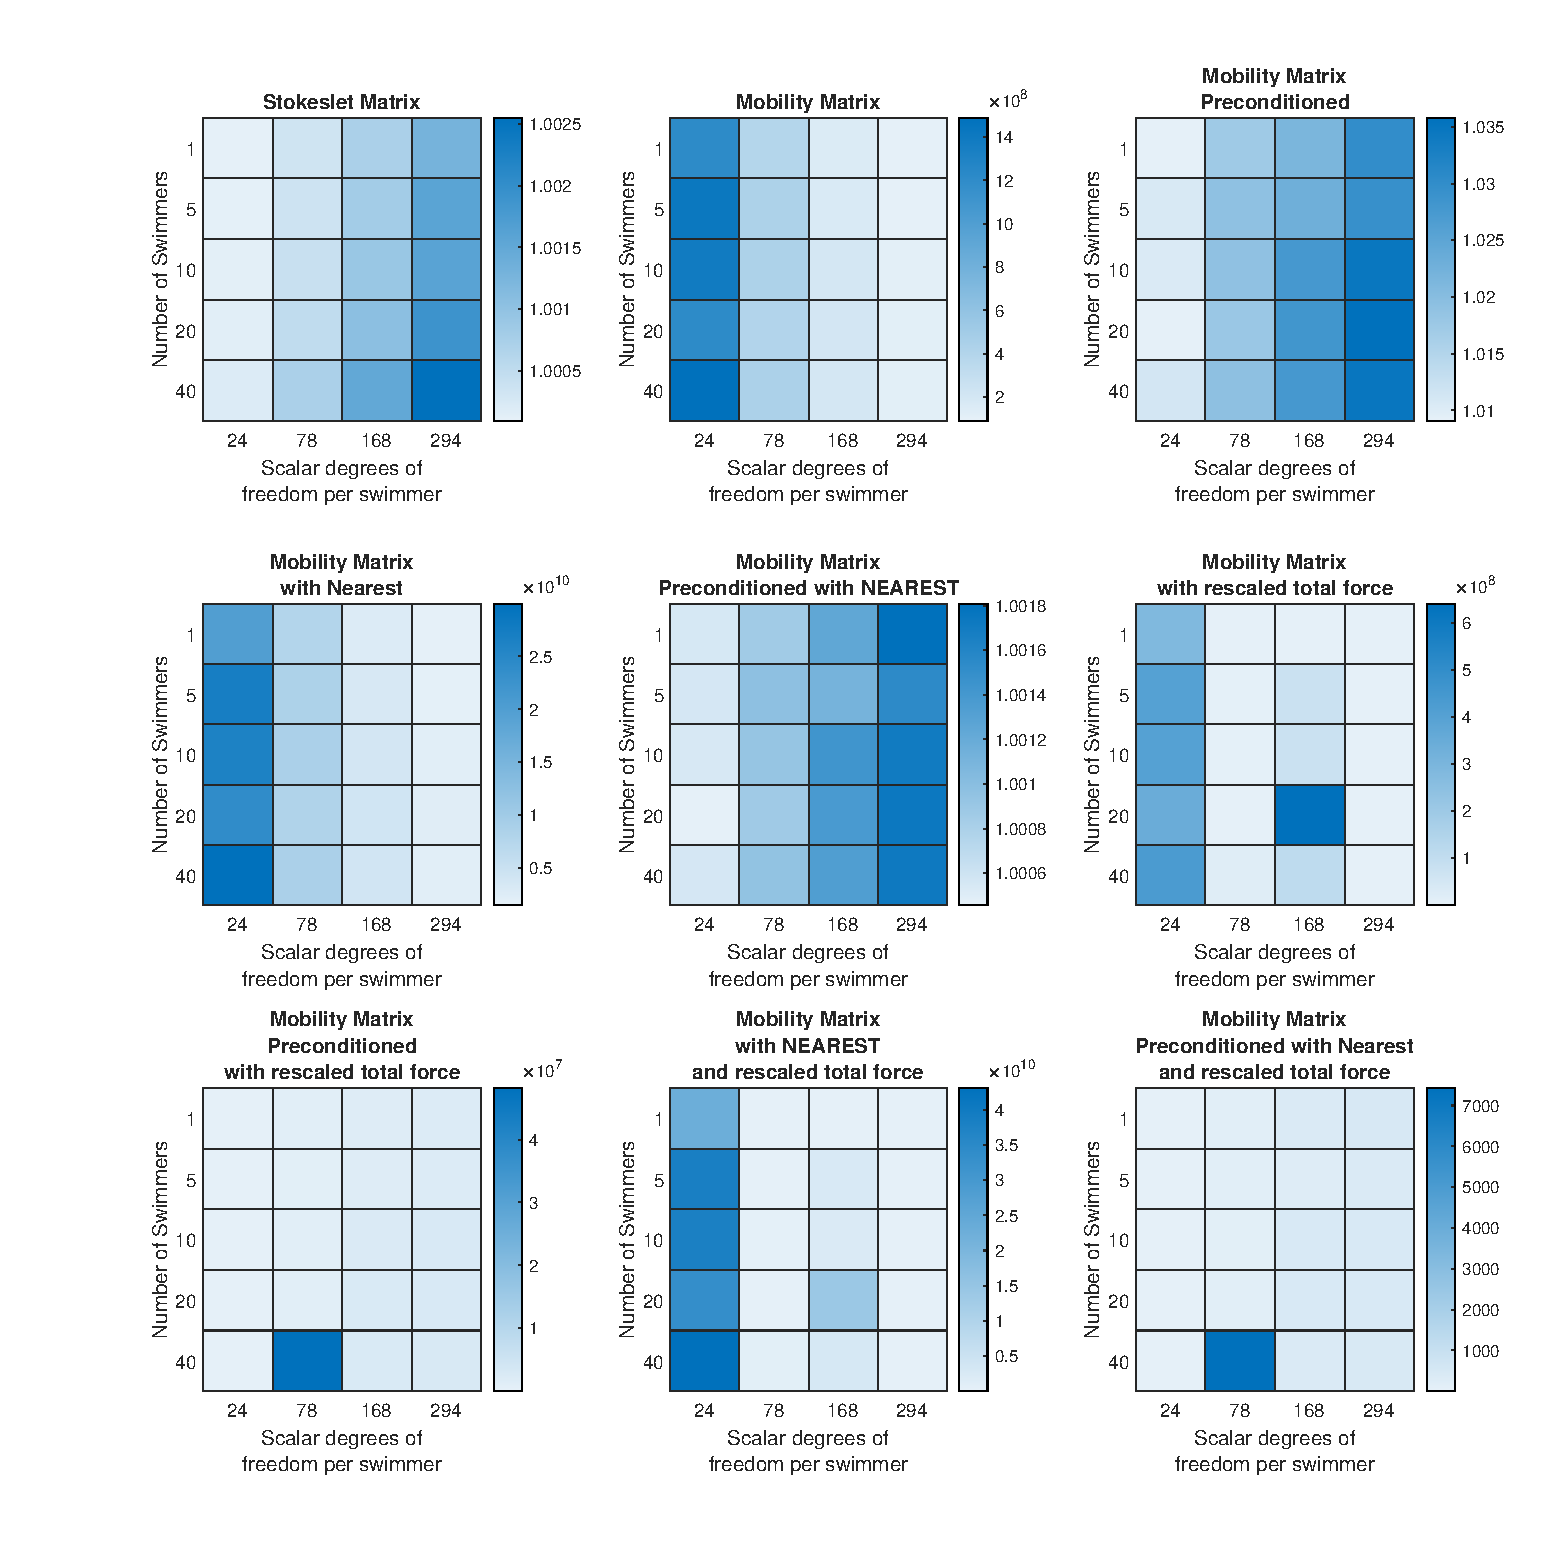
\includegraphics[height=0.49\textheight,keepaspectratio]{Images/Condition/Condition-5.pdf}
        \caption{Figure showing the condition number for various matrices shown in the paper for the case of $\epsilon=1e-5$.}
        \label{fig:Condition5}
     \end{subfigure}
    \caption{Condition number for various matrices shown in the paper}
\end{sidewaysfigure}


 \begin{sidewaysfigure}[!htbp]
     \centering
     \begin{subfigure}[b]{0.49\textwidth}
        \captionsetup{width=0.49\textwidth}
        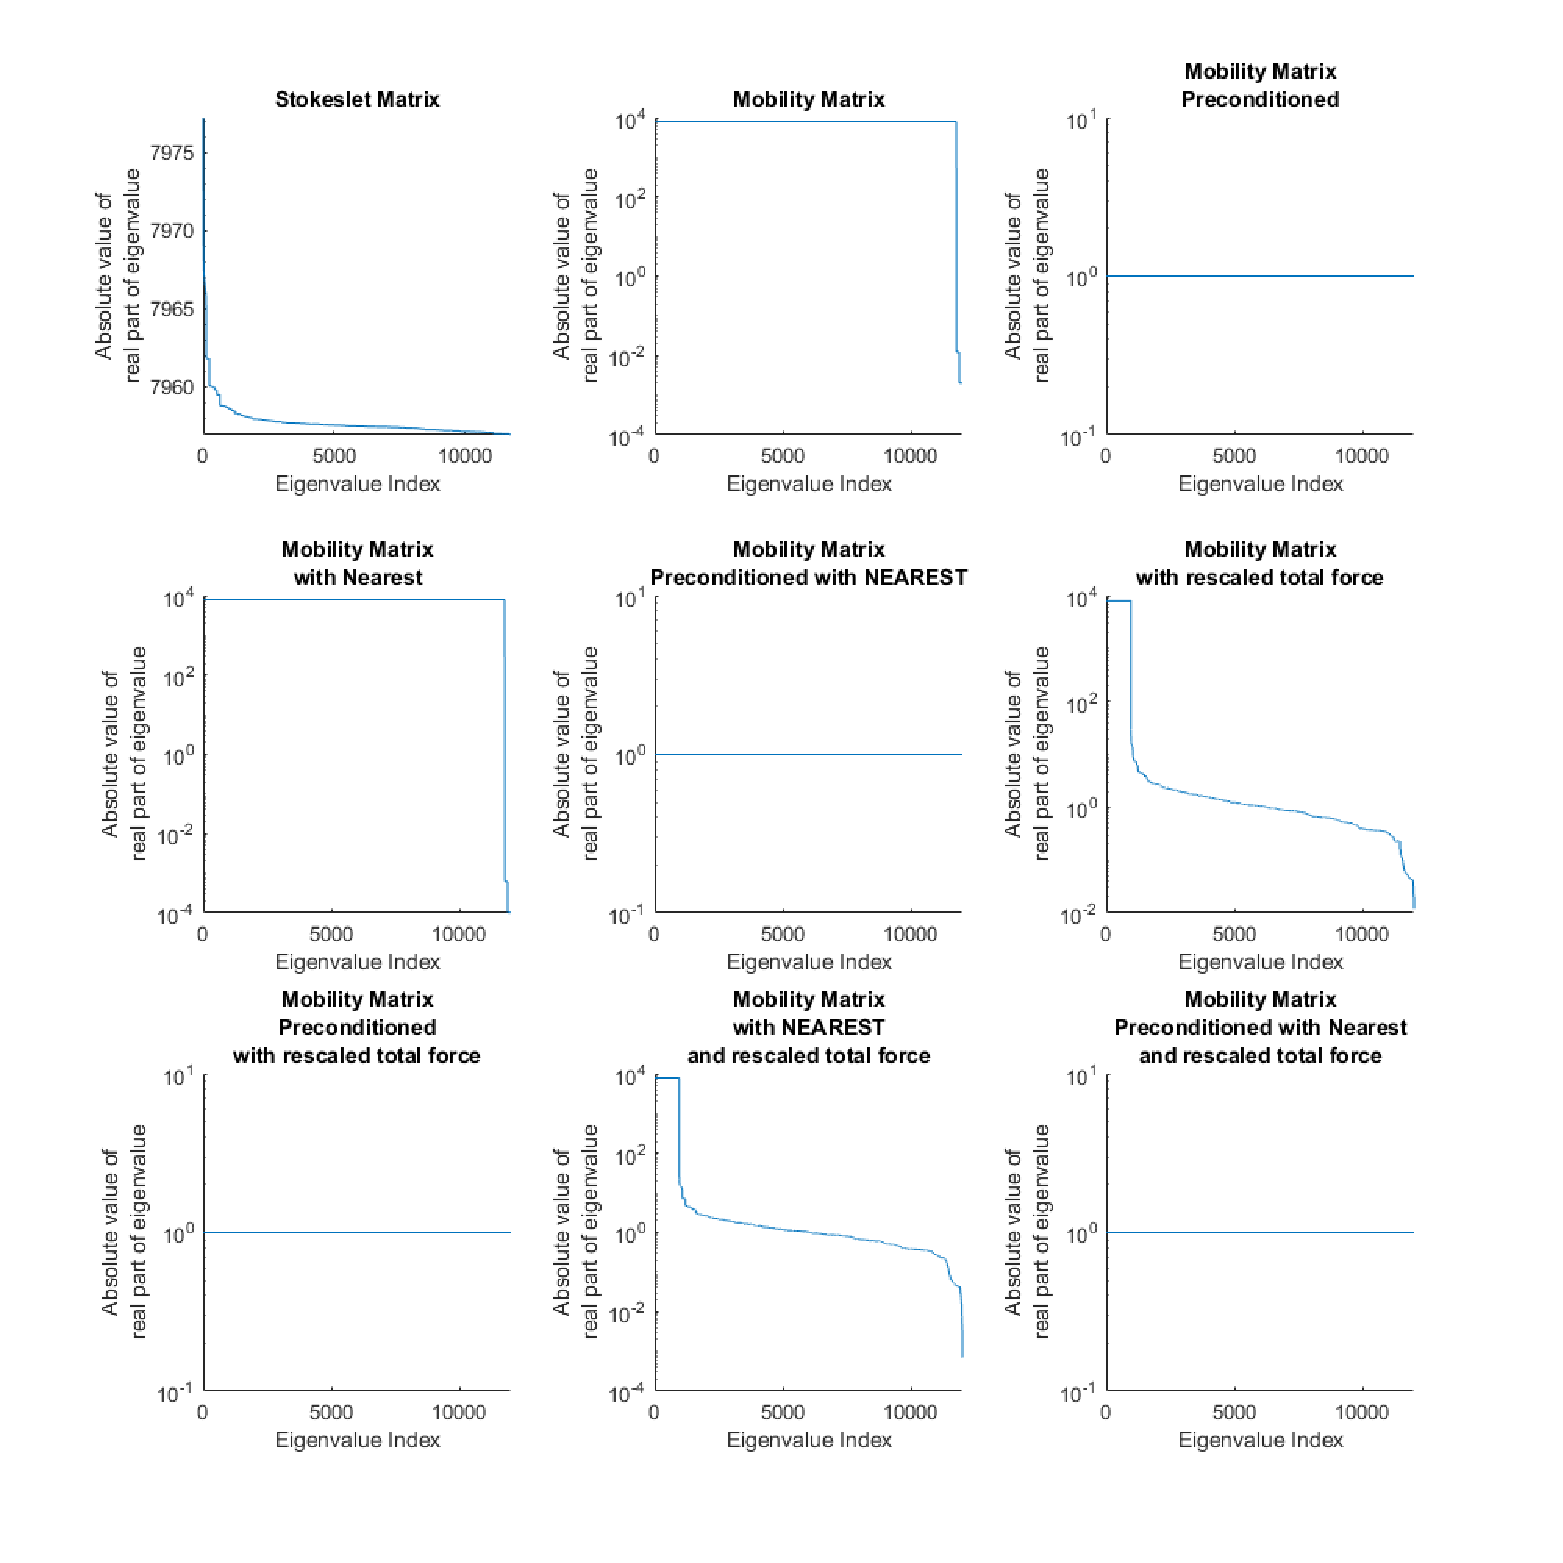
\includegraphics[height=0.49\textheight,keepaspectratio]{Images/Eigenplots/EigenPlots-1.pdf}
        \caption{Caption}
        \label{fig:Eigen1}
    \end{subfigure}
\end{sidewaysfigure}
\begin{sidewaysfigure}[!ht]
\ContinuedFloat
    \centering
    \begin{subfigure}[b]{0.49\textwidth}
        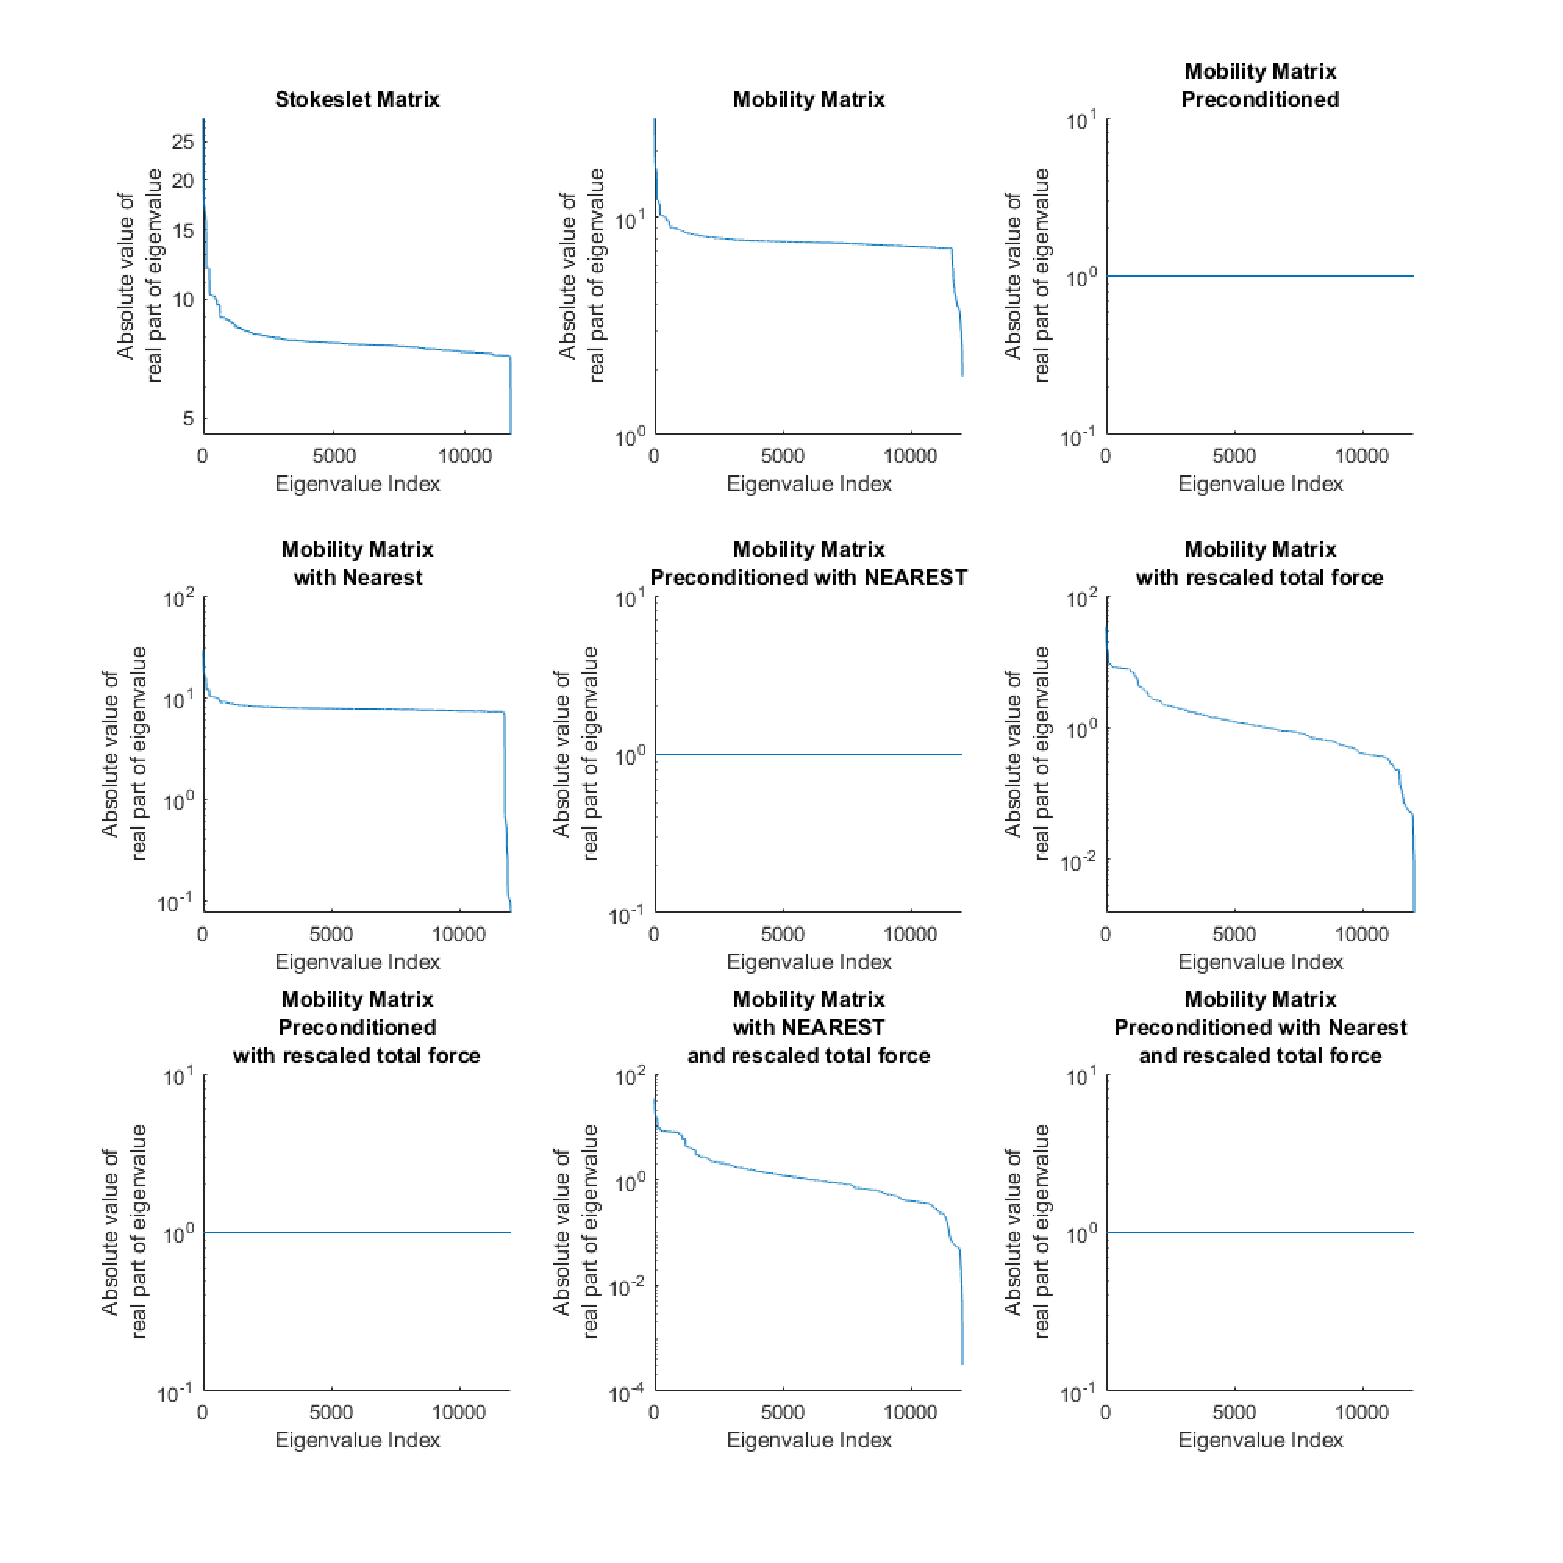
\includegraphics[height=0.49\textheight,keepaspectratio]{Images/Eigenplots/EigenPlots-2.pdf}
        \caption{Caption}
    \end{subfigure}
    \hfill
    \begin{subfigure}[b]{0.49\textwidth}
        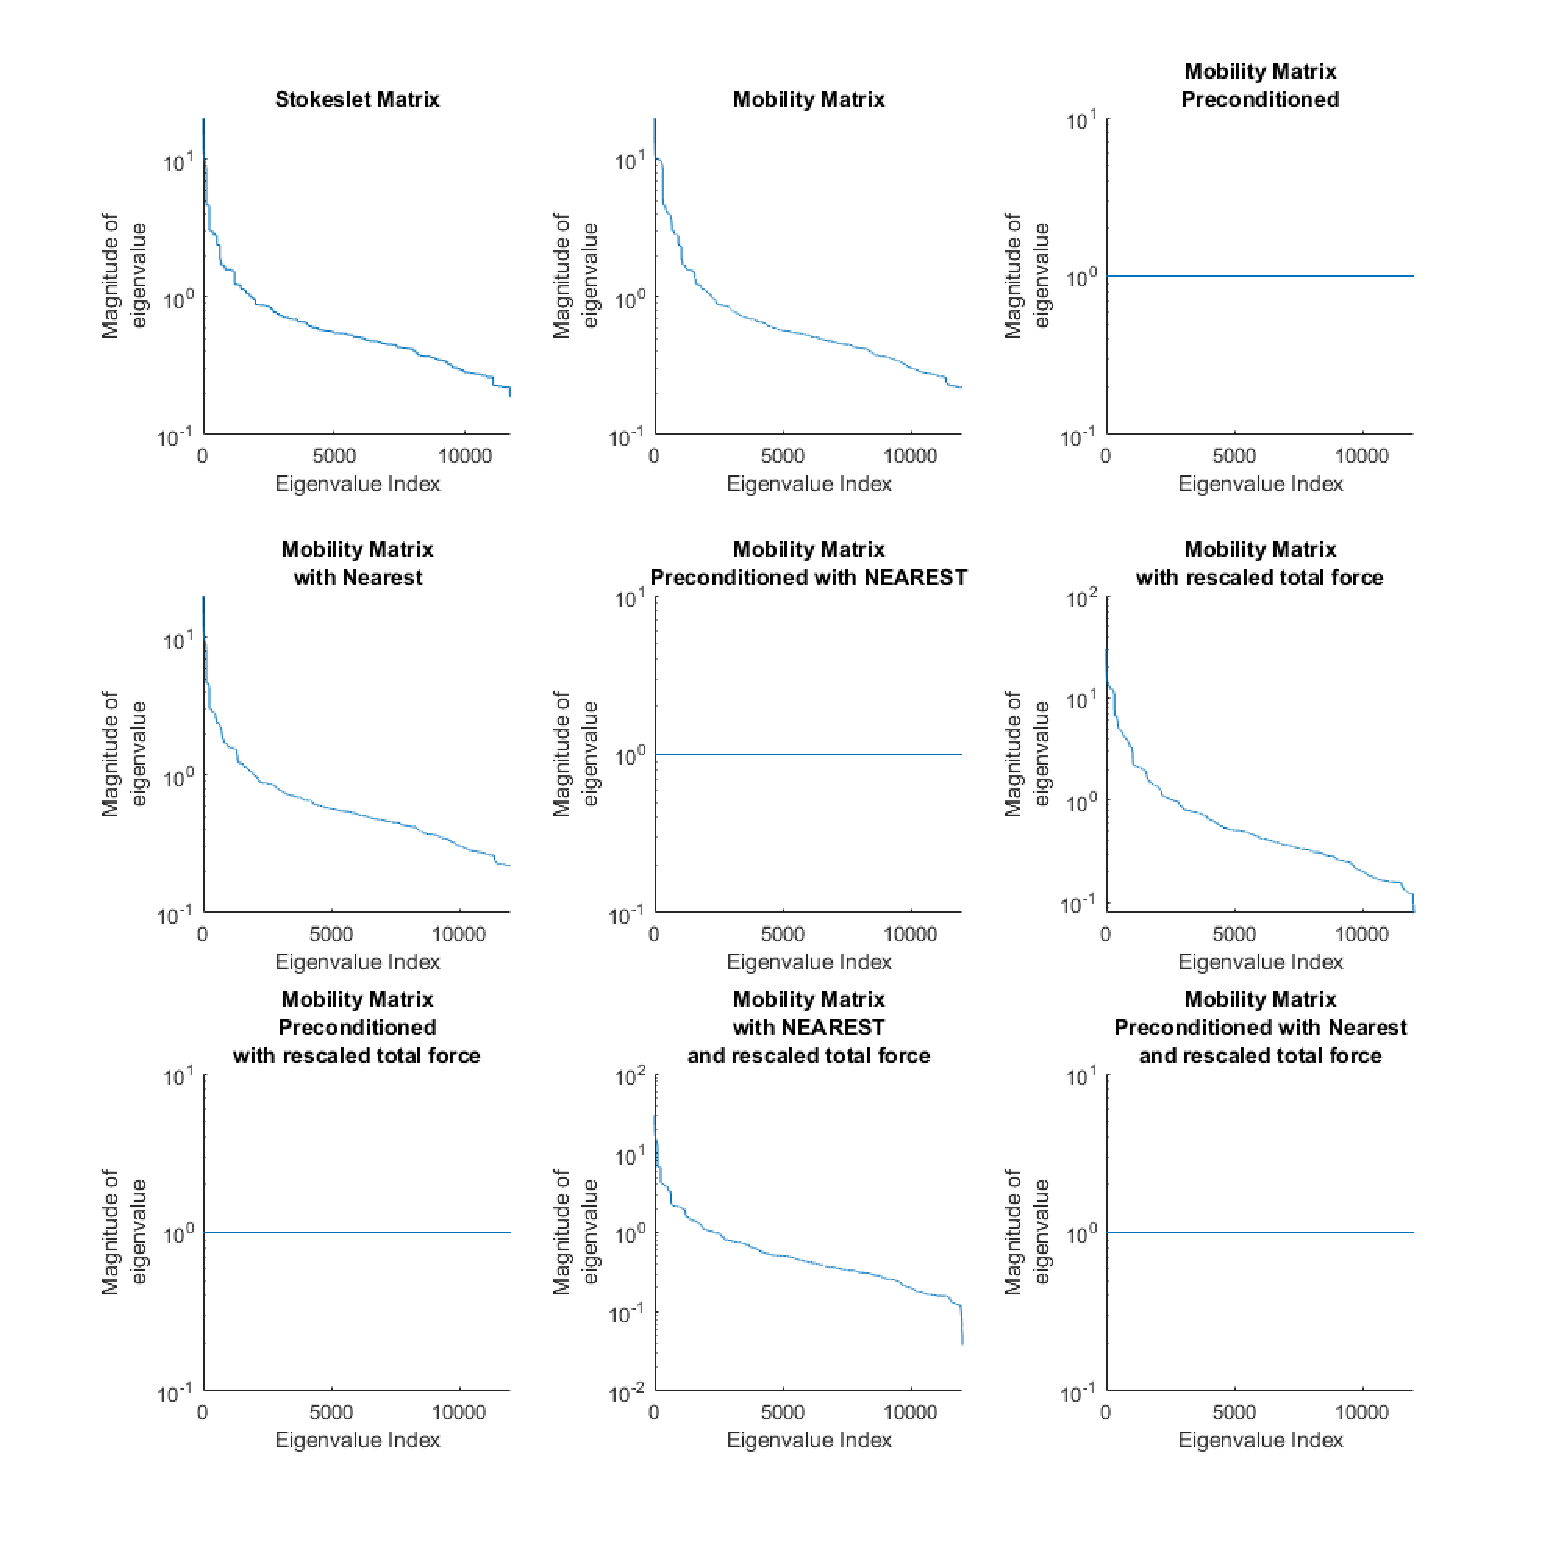
\includegraphics[height=0.49\textheight,keepaspectratio]{Images/Eigenplots/EigenPlots-5.pdf}
        \caption{Caption}
        \label{fig:Eigen5}
    \end{subfigure}
    \caption{Magnitude of eigenvalues for various matrices shown in the paper}
\end{sidewaysfigure}
\end{comment}
